\documentclass[12pt]{article}
\usepackage{amsmath}
\usepackage{graphicx}
\usepackage{enumerate}
\usepackage{natbib}
\usepackage{url}

\usepackage{amsmath,amssymb,amsthm,bm,mathtools}
\usepackage{algorithm}
\usepackage{dsfont,multirow,hyperref,setspace,enumerate}
\hypersetup{colorlinks,linkcolor={black},citecolor={blue},urlcolor={blue}}


\newcommand{\blind}{1}


\addtolength{\oddsidemargin}{-.5in}%
\addtolength{\evensidemargin}{-.5in}%
\addtolength{\textwidth}{1in}%
\addtolength{\textheight}{-.3in}%
\addtolength{\topmargin}{-.8in}%

\theoremstyle{plain}
\newtheorem{thm}{Theorem}[section]
\newtheorem{lem}{Lemma}
\newtheorem{prop}{Proposition}
\newtheorem{pro}{Property}
\newtheorem{assumption}{Assumption}
\newtheorem{cor}{Corollary}[section]

\theoremstyle{definition}
\newtheorem{defn}{Definition}
\newtheorem{example}{Example}
\newtheorem{rmk}{Remark}

\usepackage{appendix}
\usepackage{wrapfig}
\mathtoolsset{showonlyrefs}

\input macros.tex



\usepackage[english]{babel}

\newcommand*{\KeepStyleUnderBrace}[1]{%f
  \mathop{%
    \mathchoice
    {\underbrace{\displaystyle#1}}%
    {\underbrace{\textstyle#1}}%
    {\underbrace{\scriptstyle#1}}%
    {\underbrace{\scriptscriptstyle#1}}%
  }\limits
}
\usepackage{xr}


\usepackage{algpseudocode,algorithm}
\algnewcommand\algorithmicinput{\textbf{Input:}}
\algnewcommand\algorithmicoutput{\textbf{Output:}}
\algnewcommand\INPUT{\item[\algorithmicinput]}
\algnewcommand\OUTPUT{\item[\algorithmicoutput]}

\def\ci{\perp\!\!\!\perp}

\def\fixme#1#2{\textbf{\color{red}[FIXME (#1): #2]}}
\begin{document}



\def\spacingset#1{\renewcommand{\baselinestretch}%
{#1}\small\normalsize} \spacingset{1}


%%%%%%%%%%%%%%%%%%%%%%%%%%%%%%%%%%%%%%%%%%%%%%%%%%%%%%%%%%%%%%%%%%%%%%%%%%%%%%

\if1\blind
{
  \title{\bf Supervised Tensor Decomposition with Interactive Side Information}
  %\author{Jiaxin Hu, Zhuoyan Xu, and Miaoyan Wang\\
   % Department of Statistics, University of Wisconsin-Madison}
  \maketitle
} \fi

\if0\blind
{
  \bigskip
  \bigskip
  \bigskip
  \begin{center}
    {\LARGE\bf Supervised Tensor Decomposition with Interactive Side Information}
\end{center}
  \medskip
} \fi

\bigskip
\begin{abstract}
Higher-order tensors have received increased attention across science and engineering. While most tensor decomposition methods are developed for a single tensor observation, scientific studies often collect side information, in the form of node features and interactions thereof, together with the tensor data. Such data problems are common in neuroimaging, network analysis, and spatial-temporal modeling. Identifying the relationship between a high-dimensional tensor and side information is important yet challenging. Here, we develop a tensor decomposition method that incorporates multiple side information as interactive features. Unlike unsupervised tensor decomposition, our supervised decomposition captures the effective dimension reduction of the data tensor confined to feature space on each mode. An efficient alternating optimization algorithm is further developed. Our proposal handles a broad range of data types, including continuous, count, and binary observations. We apply the method to diffusion tensor imaging data from human connectome project and multi-relational social network data. We identify the key global connectivity pattern and pinpoints the local regions that are associated with available features. Our method will help the practitioners efficiently analyze tensor datasets in various areas. Toward this end, the package and data used are available at~\url{https://CRAN.R-project.org/package=tensorregress}.

\end{abstract}

\noindent%
{\it Keywords:} Applications and case studies, Tensor data analysis, Supervised dimension reduction, Exponential family distribution, Generalized multilinear model
\vfill

\newpage
\spacingset{1.5} % DON'T change the spacing!
\section{Introduction}
\label{sec:intro}


Multi-dimensional arrays, known as tensors, are often collected with side information on multiple modes in modern scientific and engineering studies. A popular example is in neuroimaging~\citep{sun2017store,zhou2013tensor}. The brain connectivity networks are collected from a sample of individuals, accompanied by individual characteristics such as age, gender, and diseases status (see Figure~\ref{fig:intro1}a). Another example is in the field of network analysis~\citep{baldin2018optimal,hoff2005bilinear}. A typical social network consists of nodes that represent people and edges that represent the friendships. Side information such as people’s demographic information and friendship types are often available. In both examples, it is of keen scientific interest to identify the variation in the tensor data (e.g., brain connectivities, social community patterns) that is affected by available features. These seemingly different scenarios pose a common yet challenging problem for tensor data modeling. 

In addition to the aforementioned challenges, many instances of tensor datasets consist of non-Gaussian measurements. Examples include the political interaction dataset \citep{hu2015scalable} which measures action counts between countries under various relationships, and the brain connectivity network dataset \citep{wang2019common} which is a collection of binary adjacency matrices. Classical tensor decomposition methods are based on minimizing the Frobenious norm of the reconstruction error, leading to suboptimal predictions for binary- or count-valued response variables. A number of supervised tensor methods have been proposed \citep{narita2012tensor, zhao2012higher, yu2016learning} to address the tensor regression problem in various forms (e.g.\ scalar-to-tensor regression, tensor-response regression). These methods often assume Gaussian distribution for the tensor entries, or impose random designs for the feature matrices, both of which are less suitable for applications of our interest. The gap in theory and practice suggests a great opportunity for improved modeling paradigms that better capture the complexity in tensor data with side information.

\begin{figure*}[t]
\begin{center}
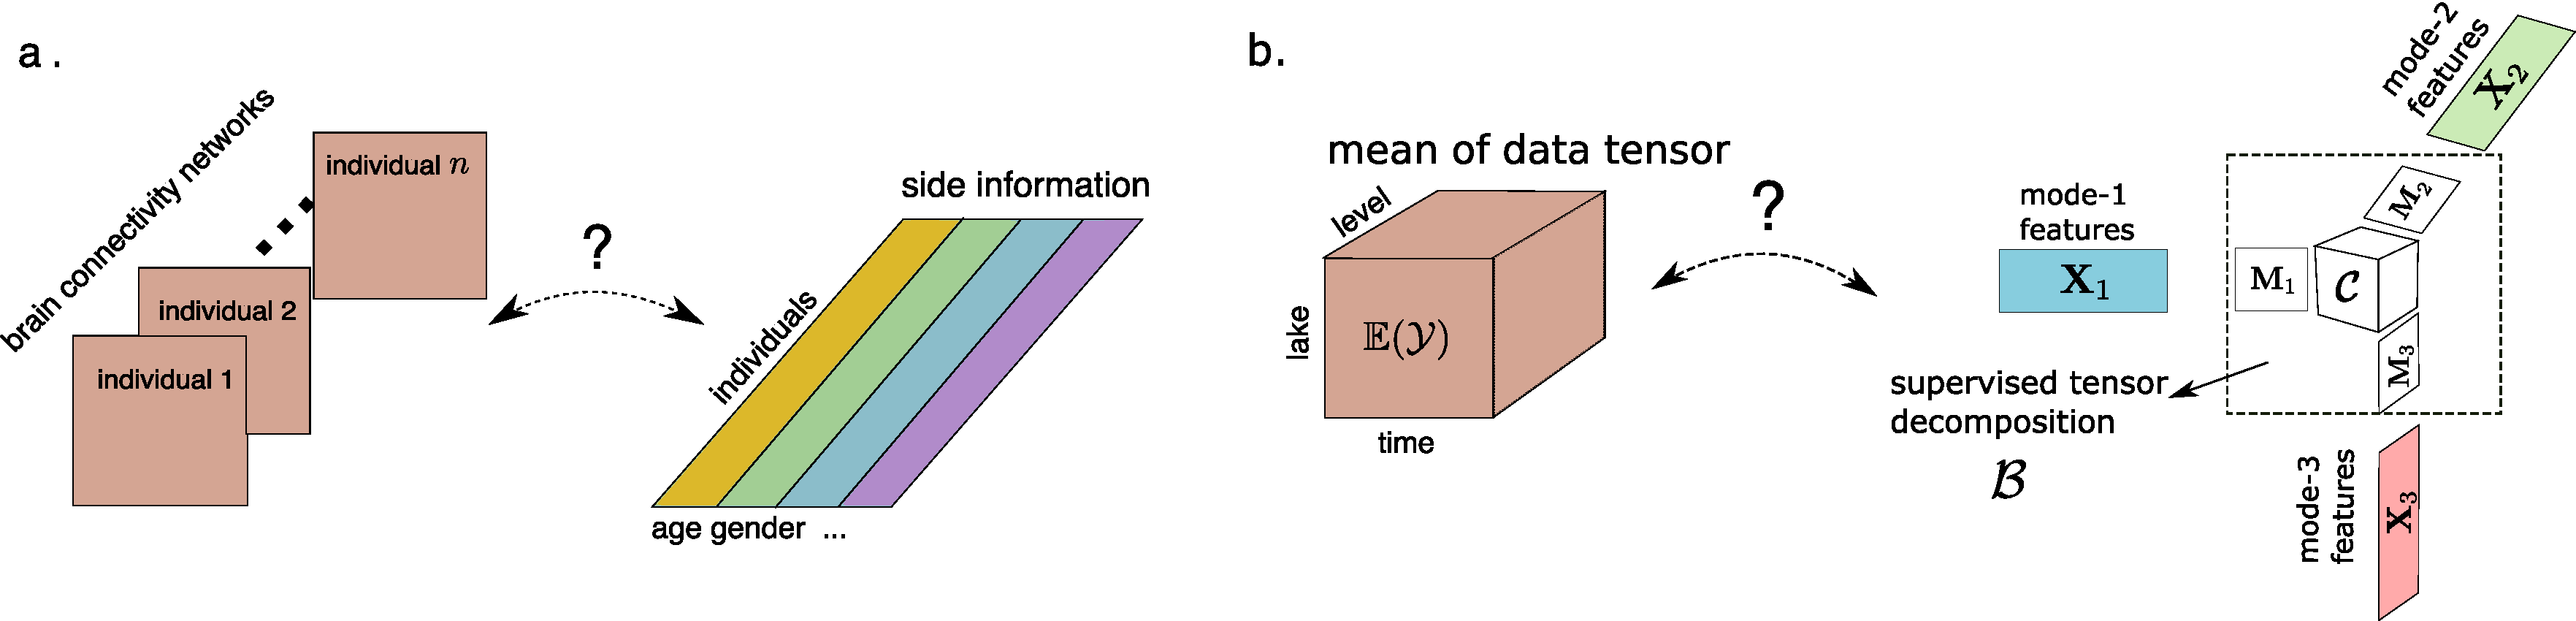
\includegraphics[width=16cm]{new_introfigure1.pdf}
\end{center}
\caption{Examples of supervised tensor decomposition with interactive side information. (a) Network population model. (b) Spatial-temporal growth model. }\label{fig:intro1}
\end{figure*}

We present a general model and associated method for decomposing a data tensor with exponential family entries and interactive side information. 
We formulate the learning task as a structured regression problem, with tensor observation serving as the response, and the multiple side information as interactive features. Figure~\ref{fig:intro1}b illustrates our model in the special case of order-3 tensors. A low-rank structure is imposed to the conditional mean tensor, where unlike classical decomposition, the tensor factors $\mX_k\mM_k\in\mathbb{R}^{d_k\times r_k}$ belong to the space spanned by features $\mX_k\in\mathbb{R}^{d_k\times p_k}$ for $k=1,2,3$. The unknown matrices $\mM_k\in\mathbb{R}^{p_k\times r_k}$ (referred to as ``dimension reduction matrices'') link the conditional mean to the feature spaces, thereby allowing the identification of variations in the tensor data attributable to the side information.

In addition, we use tools from generalized linear model (GLM) to allow heteroscedacity due to the mean-variance relationship in the non-Gaussian data. This flexibility is important in practice. In classical GLM, the sample size and feature dimension are well defined; however, in the tensor data analysis, we observe only one single realization of tensor response but up to $K$ interactive feature matrices, where $K$ is the number of tensor modes. Both the sample size and feature dimension grow exponentially in $K$. We use a low-rank constraint in the conditional mean tensor (with a suitable transformation) to mitigate the curse of high dimensionality. The statistical convergence of our estimator is established, and we quantify the gain in prediction through several case studies. 
 
Our work is closely related to but also clearly distinctive from several lines of previous work. The first line is a class of \textit{unsupervised} tensor decomposition such as Tucker and CP decomposition~\citep{de2000multilinear, kolda2009tensor,zhang2018tensor, hong2020generalized} that aims to find the best low-rank representation of a data tensor. In contrast, our model is a \textit{supervised} tensor learning, which aims to identify the association between a data tensor and multiple features. The low-rank factorization is determined jointly by the tensor data and feature matrices.

The second line of work studies the scalar-to-tensor regression, in which the response is a scalar and the predictor is a tensor~\citep{zhou2013tensor,chen2019non}. Our proposal is orthogonal to this line because we treat the data tensor as random variables. The difference in model settings yields different focuses and interpretations. Consider the neuroimaging analysis as an example. The scalar-to-tensor regression aims to predict the people's disease status based on brain connectivity network, while tensor-to-scalar model focuses on understanding the variation in the brain connectivity attributable to the individual features such as age, gender, and disease status. The scalar-to-tensor model is insufficient for tensor dimension reduction because it lacks the modeling of stochastic noise in the data tensor. 

The third line of work studies the tensor-on-tensor regression, in which both the response and predictor are tensors~\citep{raskutti2015convex, lock2018tensor, gahrooei2020multiple}. Our model shares a common ground but provides a more efficient context-specific solutions than earlier approaches. As we show in Section~\ref{subsec:statprob}, the supervised tensor decomposition 
has an interesting interpretation as a special tensor-on-tensor regression. Nevertheless, our work improves from previous work in scope and applicability. Previous methods~\citep{gahrooei2020multiple,lock2018tensor} mainly focus on Gaussian tensors. The Frobenius norm used in the objective function is statistical suboptimal for general exponential family tensors. Maximum likelihood estimator (MLE) is studied in~\cite{raskutti2015convex} and a convex relaxation algorithm is proposed to solve for low-rank tensor coefficients. However, in the tensor case, convex MLE suffers from both computational intractability and statistical suboptimality. We advocate a non-convex approach and provide strong evidence for its success in our setting. Most previous tensor regression focuses on prediction~\citep{lock2018tensor,raskutti2015convex,gahrooei2020multiple}, and we go step further by finding the sufficient dimension reduction~\citep{adragni2009sufficient}, $\text{Span}(\mM_k)$, that facilitates the identification of effective features in prediction (see Figure~\ref{fig:intro1}b). The latter approach greatly improves the \emph{interpretability} in prediction. In this regards, our method opens up new opportunities for tensor data analysis in a wider range of possible applications. 

\fixme{Miaoyan}{One more paragraph. Current literature on tensor decomposition with auxiliary side information...}

The remainder of this paper is organized as follows. Section~\ref{sec:pre} introduces tensor notation and preliminaries. Section~\ref{sec:model} presents the main model and three motivating examples for supervised tensor decomposition. Section~\ref{sec:est} describes a rank-constrained likelihood-based estimation and associated alternating optimization algorithm. In Section~\ref{sec:simulation}, we present numerical experiments and assess the performance in comparison to alternative methods. In Section~\ref{sec:data}, we apply the method to diffusion tensor imaging data from human connectome project and multi-relational social network data. We conclude in Section~\ref{sec:con} with discussions about our findings and avenues of future work.

\section{Preliminaries}\label{sec:pre}

We introduce the basic tensor properties used in the paper; more details on tensor notation can be found in~\citet{kolda2009tensor}. We use $\tY=\entry{y_{i_1,\ldots,i_K}}\in \mathbb{R}^{d_1\times \cdots\times d_K}$\fixme{Miaoyan}{perhaps use $y_\omega$} to denote an order-$K$ $(d_1,\ldots,d_K)$-dimensional tensor, where $K$ corresponds to the number of modes of $\tY$ and is called the order. The multilinear multiplication of a tensor $\tY\in\mathbb{R}^{d_1\times \cdots\times d_K}$ by matrices $\mX_k=\entry{x_{i_k,j_k}^{(k)}}\in\mathbb{R}^{p_k\times d_k}$ is defined as
\begin{equation}
\tY \times_1\mX_1\ldots \times_K \mX_K=\entry{\sum_{i_1,\ldots,i_K}y_{i_1,\ldots,i_K}x_{j_1,i_1}^{(1)}\ldots x_{j_K,i_K}^{(K)}},
\end{equation}
which results in an order-$K$ $(p_1,\ldots,p_K)$-dimensional tensor. For ease of presentation, we use the shorthand $\tY\times\{\mX_1,\ldots,\mX_K\}$ to denote the tensor-by-matrix product. For any two tensors $\tY=\entry{y_{i_1,\ldots,i_K}}$, $\tY'=\entry{y'_{i_1,\ldots,i_K}}$ of identical order and dimensions, their inner product is defined as 
\[
\langle \tY,\ \tY'\rangle =\sum_{i_1,\ldots,i_K}y_{i_1,\ldots,i_K}y'_{i_1,\ldots,i_K}.
\] 
The Frobenius norm and maximum norm of $\tY$ are defined as 
\[
\FnormSize{}{\tY}=\langle \tY,\ \tY \rangle^{1/2}\quad \text{and}\quad \mnormSize{}{\tY}=\max_{i_1,\ldots,i_K}y_{i_1,\ldots,i_K}.
\]
 A higher-order tensor can be reshaped into a lower-order object. We use $\text{vec}(\cdot)$ to denote the operation that reshapes the tensor into a vector, and $\text{Unfold}_k(\cdot)$ the operation that reshapes the tensor along mode-$k$ into a matrix of size $d_k$-by-$\prod_{i\neq k}d_i$. The multilinear rank of an order-$K$ tensor $\tY$ is defined as a length-$K$ vector $\mr=(r_1,\ldots,r_K)$, where $r_k$ is the rank of matrix $\text{Unfold}_k(\tY)$, $k=1,\ldots,K$. Given a matrix $\mM\in\mathbb{R}^{d\times r}$, we use $\text{Span}(\mM)$ to denote the space spanned by columns of $\mM$. We use lower-case letters (e.g.,\ $a,\ b,\ c$) for scalars and vectors, upper-case boldface letters (e.g.,\ $\mA,\ \mB,\ \mC$) for matrices, and calligraphy letters (e.g.,\ $\tA,\ \tB,\  \tC$) for tensors of order three or greater. We let $\mI_d$ denote the $d \times d$ identity matrix and $[d]$ denote the $d$-set $\{1,\ldots,d\}$. For ease of notation, we allow the basic arithmetic operators (e.g.,\ $+$, $-$, $\geq $) and univariate 
functions $f\colon \mathbb{R}\to \mathbb{R}$ to be applied to tensors in an element-wise manner.

\section{Motivation and model}\label{sec:model}
\subsection{General framework for supervised tensor decomposition}
We begin with a general framework for supervised tensor decomposition and then discuss its implication in three concrete examples. Let $\tY=\entry{y_{i_1,\ldots,i_K}}\in\mathbb{R}^{d_1\times \cdots\times d_K}$ denote an order-$K$ data tensor. Suppose the side information is available on each of the $K$ modes. Let $\mX_k=\entry{x_{ij}}\in\mathbb{R}^{d_k\times p_k}$ denote the feature matrix on the mode $k\in[K]$, where $x_{ij}$ denotes the $j$-th feature value for the $i$-th tensor entity, for $(i,j)\in[d_k]\times[p_k]$, $p_k\leq d_k$. We propose a multilinear conditional mean model between the data tensor and feature matrices. Assume that, conditional on the features $\mX_k$, the entries of tensor $\tY$ are independent realizations from an exponential family distribution, and the conditional mean tensor admits the form
\begin{align}\label{eq:tensormodel}
&\mathbb{E}(\tY|\mX_1,\ldots,\mX_K)=f(\Theta),\quad \text{with}\quad \Theta =\tB\times\{\mX_1,\ \ldots,\ \mX_K\} ,
\end{align}
where $\Theta\in\mathbb{R}^{d_1\times \cdots\times d_K}$ is the multilinear predictor, $\tB\in\mathbb{R}^{p_1\times \cdots \times p_K}$ is the unknown parameter tensor, $f(\cdot)$ is a known link function whose form depending on the data type of $\tY$, and $\times$ denotes the tensor-by-matrix product. The choice of link function is based on the assumed distribution family of tensor entries. Common choices of link functions include identity link for Gaussian distribution, logistic link for Bernoulli distribution, and $\exp(\cdot)$ link for Poisson distribution. In general, dispersion parameters can also be included in the model. Because our main focus is the tensor decomposition under the mean model, we omit the dispersion parameter in this section for ease of presentation. 


In classical tensor decomposition, tensor factorization is performed on either data tensor $\tY$ or mean tensor $\mathbb{E}(\tY)$. In the context of supervised tensor decomposition, we propose to factorize the latent parameter tensor $\tB$,
\begin{equation}\label{eq:factor}
\tB=\tC\times\{\mM_1,\ \ldots,\ \mM_K\},
\end{equation}
where $\tC\in\mathbb{R}^{r_1\times \cdots \times r_K}$ is a full-rank core tensor, and $\mM_k\in\mathbb{R}^{p_k\times r_k}$ are factor matrices consisting of orthonormal columns, where $r_k\leq p_k$ for all $k\in[K]$. By the definition of multilinear rank, model equations~\eqref{eq:tensormodel} and~\eqref{eq:factor} imply the low-rankness $\mr=(r_1,\ldots,r_K)$ of the conditional mean tensor under the link function. We now reach our final model for supervised tensor decomposition,
\begin{align}\label{eq:decomp}
\mathbb{E}(\tY|\mX_1,\ldots,\mX_K) &= f\left(\tC\times\{\mX_1\mM_1,\ \ldots,\ \mX_K\mM_K\}\right),\notag\\
\text{where} \ &\ \mM_k\mM^T_k=\mI_{p_k},\ \mM_k\in\mathbb{R}^{p_k\times r_k}\ \text{for all }k=1,\ldots,K,
\end{align}
where the parameters of interest are $\mM_k$ and $\tC$. Note that model~\eqref{eq:decomp} assumes a fixed, known rank $\mr=(r_1,\ldots,r_K)$; the adaptation to unknown rank will be addressed in Section~\ref{sec:tuning}. Figure~\ref{fig:intro1}b provides a schematic illustration of our model. The features $\mX_k$ affect the distribution of tensor entries in $\tY$ through the form $\mX_k\mM_k$, which are $r_k$ linear combinations of features on mode $k$. We call $\mX_k\mM_k$ the ``supervised tensor factors'' or ``sufficient features''~\citep{adragni2009sufficient}, and call $\mM_k$ the ``dimension reduction matrix.'' The core tensor $\tC$ collects the interaction effects between sufficient features across $K$ modes. Our goal is to find $\mM_k$ and the corresponding $\tC$. Note that $\mM_k$ and $\tC$ are identifiable only up to orthonormal transformations.  



\subsection{Three examples}
We give three concrete examples of supervised tensor decomposition model~\eqref{eq:decomp} that arises in practice. 
\begin{example}[Spatio-temporal growth model]
The growth curve model~\citep{gabriel1998generalised,potthoff1964generalized,srivastava2008models} was originally proposed as an example of bilinear model for matrix data, and we adopt its higher-order extension here. Let $\tY=\entry{y_{ijk}}\in\mathbb{R}^{d \times m\times n}$ denote the pH measurements of $d$ lakes at $m$ levels of depth and for $n$ time points. Suppose the sampled lakes belong to $q$ types, with $p$ lakes in each type. Let $\{\ell_j\}_{j\in[m]}$ denote the sampled depth levels and $\{t_k\}_{k\in[n]}$ the time points. Assume that the expected pH trend in depth is a polynomial of order at most $r$ and that the expected trend in time is a polynomial of order $s$. Then, the conditional mean model for the spatio-temporal growth model can be represented as
\begin{equation}\label{eq:time}
\mathbb{E}(\tY|\mX_1,\mX_2,\mX_3)=\tC\times\{\mX_1\mM_1,\ \mX_2\mM_2,\ \mX_3\mM_3\},
\end{equation}
where $\mX_1=\text{blockdiag}\{\mathbf{1}_p,\ldots,\mathbf{1}_p\}\in \{0,1\}^{d\times q}$ is the design matrix for lake types, and
\[
\mX_2=
\begin{pmatrix}
1 & \ell_1&\cdots &\ell^{r}_1\\
1 & \ell_2&\cdots &\ell^{r}_2\\
\vdots &\vdots&\ddots&\vdots\\
1&\ell_{m}&\cdots&\ell^{r}_{m}
\end{pmatrix},\quad
\mX_3=
\begin{pmatrix}
1 & t_1&\cdots &t^{s}_1\\
1 & t_2&\cdots &t^{s}_2\\
\vdots &\vdots&\ddots&\vdots\\
1&t_{n}&\cdots&t^{s}_{n}
\end{pmatrix}
\]
are the design matrices for spatial and temporal effects, respectively, $\tC\in\mathbb{R}^{r_1\times r_2\times r_3}$ is the unknown core tensor, and $\mM_k$ are unknown dimension reduction matrices of coherent sizes. The factors $\mX_k\mM_k$ are sufficient features for the mean model~\eqref{eq:time}. The spatial-temporal model is a special case of our supervised tensor decomposition model, with features available on each of the three modes.
\end{example}


\begin{example}[Network population model]\label{example:brain}
Network response model~\citep{rabusseau2016low, zhang2018network} is recently developed for neuroimanig analysis. The goal is to study the relationship between brain network connectivity pattern and features of individuals. Suppose we have a sample of $n$ observations, $\{(\mY_i, \mx_i)\colon i=1,\ldots,n\}$, where for each individual $i\in[n]$, $\mY_i\in\{0,1\}^{d\times d}$ is the symmetric adjacency matrix whose entries indicate presences/absences of connectivities between $d$ brain nodes, and $\mx_i\in\mathbb{R}^p$ is the individual's feature such as age, gender, cognition score, etc. The network-response model  has the conditional mean
\begin{equation}\label{eq:network}
\text{logit}(\mathbb{E}(\mY_i|\mx_i))=\tB\times_3\mx_i, \quad \text{for }i=1,\ldots,n,
\end{equation}
where $\tB\in \mathbb{R}^{d\times d\times p}$ is a coefficient tensor of rank $r(\tB)=(r,r,r')$.

The model~\eqref{eq:network} is a special case of our supervised tensor decomposition, with feature matrix on the last mode of the tensor. Specifically, we stack the network observations $\{\mY_i\}$ together and obtain an order-3 response tensor $\tY\in\{0,1\}^{d\times d\times n}$. Define a feature matrix $\mX=[\mx_1,\ldots,\mx_n]^T\in\mathbb{R}^{n\times p}$. Then, the model~\eqref{eq:network} has the equivalent representation of supervised tensor decomposition,
\[
\text{logit}(\mathbb{E}(\tY|\mX))=\tC\times\{\mM,\ \mM,\ \mX\mM'\},
\]
where $\tC\in\mathbb{R}^{r\times r\times r'}$ is the core tensor, $\mM\in\mathbb{R}^{d\times r}$ is the dimension reduction matrix at the first two modes, and $\mM'\in\mathbb{R}^{p\times r'}$ is for the last mode.  \end{example}
 
 \begin{example}[Dyadic data with node attributes] Dyadic dataset consists of measurements on pairs of objects or under a pair of conditions. Common examples include graphs and networks. Let $\tG=(V,E)$ denote a graph, where $V=[d]$ is the node set of the graph, and $E\subset V\times V$ is the edge set. Suppose that we also observe feature vector $\mx_i\in\mathbb{R}^p$ associated to each $i\in V$. A probabilistic model on the graph $\tG=(V,E)$ can be described by the following matrix regression. The edge connects the two vertices $i$ and $j$ independently of other pairs, and the probability of connection is modeled as
\begin{equation}\label{eq:edge}
 \text{logit}\left(\mathbb{P}\left((i,j)\in E\right)\right)=\mx^T_i\mB\mx_j=\langle \mB,\ \mx^T_i\mx_j\rangle,
 \end{equation}
 where $\mB\in\mathbb{R}^{p\times p}$ is a symmetric rank-$r$ matrix. The low-rankness in $\mB$ has demonstrated its success in modeling transitivity, balance, and communities in the networks~\citep{hoff2005bilinear}. We show that our supervised tensor decompostiion~\eqref{eq:tensormodel} also incorporates the graph model as a special case. Let $\tY=\entry{y_{ij}}$ be a binary matrix where $y_{ij}=\mathds{1}_{(i,j)\in E}$. Define $\mX=[\mx_1,\ldots,\mx_n]^T\in\mathbb{R}^{n\times p}$. Then, the graph model~\eqref{eq:edge} can be expressed as
 \[
 \text{logit}(\mathbb{E}(\mY|\mX))=\mC\times\{\mX\mM,\ \mX\mM\}, 
  \]
  where $\mC\in\mathbb{R}^{r\times r}$ and $\mM\in\mathbb{R}^{p\times r}$ are based on the singular value decomposition of $\mB=\mM\mC\mM^T$. 
  \end{example}


In the above three examples and many other studies, researchers are interested in uncovering the variation in the data tensor that can be explained by features. 
%The core tensor $\tC$ in our model model~\eqref{eq:tensormodel} serves this goal by collecting the sufficient feature effects and the interaction thereof.  
\fixme{Miaoyan}{Unclear... To encourage the sharing among effects, decomposition~\eqref{eq:factor} assumes that the feature effects $\tB$ lie in a low-dimensional parameter space.
%\begin{equation}\label{eq:rank}
%\small \tP_{r_1,\ldots,r_K}=\{\tB\in\mathbb{R}^{p_1\times \cdots \times p_K}: r_k(\tB)\leq r_k \text{ for all } k\in[K]\},
%\end{equation}
%where $r_k(\tB)\leq p_k$ is the rank at mode $k$ of the tensor. 
The low-rank assumption is plausible in many scientific applications. In the Example~\ref{example:brain} of brain imaging analysis, for instance, it is often believed that the brain nodes can be partitioned into several functional and structural regions, and the person's attribute effect the connectivity in a similar way within a region. }

%{\color{red}The low-rank structure encourages the shared information across tensor entries, thereby greatly improving the estimation stability. }
%When no confusion arises, we drop the subscript $(r_1,\ldots,r_K)$ and write $\tP$ for simplicity.

Our supervised tensor decomposition~\eqref{eq:decomp} is able to incorporate arbitrary numbers of feature matrices. We set $\mX_k=\mI_{d_k}$ if certain mode $k$ has no available side information. In particular, our model~\eqref{eq:decomp} reduces to classical unsupervised tensor decomposition~\citep{de2000multilinear,hong2018generalized} if no side information is available; i.e., $\mX_k=\mI_{d_k}$ for all $k\in[K]$.
%Then, the final form of our tensor regression model can be written as:
%\begin{align}\label{eq:tensormodel2}
%&\mathbb{E}(\tY|\tX)=f(\Theta),\quad \Theta =\tC\times\{\mX_1\mM_k,\ldots,\mX_k\mK_k\},\notag\\
%&\text{where}\ \mM^T_k\mM_k=1
%\end{align}
%where the entriesof $\tY$ are independent random variables conditional on $\tX$, and $\tB\in\mathbb{R}^{p_1\times \cdots\times p_K}$ is the low-rank coefficient tensor of interest. 
%We comment that other forms of tensor low-rankness are also possible, and here we choose Tucker rank just for parsimony. Similar models can be derived using various notions of low-rankness based on CP decomposition~\citep{hitchcock1927expression} and train decomposition~\citep{oseledets2011tensor}. 

\subsection{Connection to sufficient dimension reduction and tensor-on-tensor regression}
An important feature of our method is that we allow high-dimensionality in both tensor dimension $d_k$ and feature dimension $p_k$. The model rank is typically smaller than tensor dimension $d_k$ and the feature dimension $p_k$. In such a case, the matrices $\mM_k$ serve the role of simultaneous dimension reduction of the data tensor and features. The implications of the sufficient features $\mX_k\mM_k$ can be seen in the following two conditional independence assumptions in model~\eqref{eq:decomp},
\begin{align}
\tY \ci \{\mX_k\}&\ \big|\ \{\mX_k\mM_k\} \ \ \text{(independence between the tensor and multiple features)},\\
y_\omega \ci y_{\omega'} & \ \big|\ \{\mX_k\mM_k\}  \ \ \text{(independence within the tensor)},
\end{align}
where the second line holds for all $\omega\neq \omega' \in[d_1]\times\cdots\times[d_K]$, and $\ci$ denotes the independence. The first property highlights the ``decorrelation'' role of $\mM_k$ akin to the sufficient dimension reduction~\citep{adragni2009sufficient} in high-dimensional supervised learning, whereas the second property highlights the tensor dimension reduction in the usual unsupervised sense (consider, for example, $\mX_k=\mathbf{I}_{d_k}$ for all $k\in[K]$).

Our model also has a close connection with tensor-on-tensor regression. Specifically, model~\eqref{eq:decomp} can be viewed as a multivariate regression model, where the response is vectorized tensor and the covariates are interactions between all sufficient features across modes. We take an order-3 tensor under the Gaussian model for illustration. Let $\mX,\mZ,\mW$ denote the feature matrix on mode $k=1, 2, 3$, respectively. Suppose that each mode has two-dimensional sufficient features, denoted $\mM_1\mX=[\mx_1,\mx_2]$, $\mM_2\mZ=[\mz_1,\mz_2]$, $\mM_3\mW=[\mw_1,\mw_2]$. Here $\mx_1,\mx_2,\ldots,\mw_1, \mw_2$ are column vectors. Then the model~\eqref{eq:decomp} can be written as a regression model with across-mode interactions,
\begin{equation}\label{eq:interaction}
\mathbb{E}(y_{ijk}|\mX,\mZ,\mW)=c_{111}\mx_{1i}\mz_{1j}\mw_{1k}+c_{121}\mx_{i1}\mz_{j2}\mw_{k1}+\cdots+c_{221}\mx_{2i}\mz_{2j}\mw_{1k}+c_{222}\mx_{2i}\mz_{2j}\mw_{2k},
\end{equation}
where $\entry{c_{ijk}} \in \mathbb{R}^{2\times 2\times 3}$ are unknown interaction effects, $\mx_{1i}$ denotes the $i$-th entry in the feature vector $\mx_1$, and similar notations apply to other features. Model~\eqref{eq:interaction} suggests the use of our supervised tensor decomposition for identifying across-mode interactions. Note that lower-order interactions are naturally incorporated in~\eqref{eq:interaction} if we include an intercept column in the sufficient feature matrices.  

\fixme{Miaoyan}{The above two aspects above two aspects in the simulation and real data analysis.}

\section{Estimation}\label{sec:est}

\subsection{Rank-constrained M-estimator}
We develop a likelihood-based procedure to estimate $\tC$ and $\mM_k$ in~\eqref{eq:decomp}. We adopt the exponential family as a flexible framework for different data types. In a classical generalized linear model (GLM) with a scalar response $y$ and feature $\mx$, the density is expressed as:
\[
p(y|\mx, \boldsymbol{\beta})=c(y,\phi)\exp\left({y\theta- b(\theta) \over \phi}\right)\ \text{with}\ \theta=\boldsymbol{\beta}^T\mx,
\]
where $b(\cdot)$ is a known function, $\theta$ is the linear predictor, $\phi>0$ is the dispersion parameter, and $c(\cdot)$ is a known normalizing function. The choice of link functions depends on the data types and on the observation domain of $y$, denoted $\mathbb{Y}$. For example, the observation domain is $\mathbb{Y}=\mathbb{R}$ for continuous data, $\mathbb{Y}=\mathbb{N}$ for count data, and  $\mathbb{Y}=\{0,1\}$ for binary data. 
Note that the canonical link function $f$ is chosen to be $f(\cdot)=b'(\cdot)$. Table~1 summarizes the canonical link functions for common types of distributions. 

\begin{table}[htb]
\centering
\begin{tabular}{c|ccc}
Data type &Gaussian & Poisson& Bernoulli\\
\hline
Domain $\mathbb{Y}$& $\mathbb{R}$&$\mathbb{N}$&$\{0,1\}$\\
 $b(\theta)$&$\theta^2/2$& $\exp(\theta)$&$\log (1+\exp(\theta))$\\
 link $f(\theta)$&$\theta$&$\exp(\theta)$&$(1+\exp(-\theta))^{-1}$
\end{tabular}
\caption{Canonical links for common distributions.}\label{table:link}
\end{table}


In our context, we model the the entries in the response tensor $y_{ijk}$ conditional on $\theta_{ijk}$ as independent draws from an exponential family. The quasi log-likelihood of~\eqref{eq:decomp} is equal (ignoring constant) to Bregman distance between $\tY$ and $b'(\Theta)$:
\begin{align}
\tL_{\tY}(\tC,\mM_k)&=\langle \tY, \Theta \rangle - \sum_{i_1,\ldots,i_K} b(\theta_{i_1,\ldots,i_K}),\\
\text{where}\ \Theta&=\tC\times\{\mM_1\mX_1,\ldots,\mM_K\mX_K\}.
\end{align}

We consider a constrained maximum likelihood estimator (M-estimator),
\begin{align} \label{eq:MLE} 
(\hat \tC, \hat \mM_1,\ldots,\hat \mM_k) &=\argmax_{(\tC,\mM_1,\ldots,\mM_K)\in \tP} \ \tL_{\tY}(\tC,\mM_1,\ldots,\mM_K),
\end{align}
where the parameter space $\tP$ is described as
\[
\tP=\left\{\tC\in\mathbb{R}^{r_1\times \cdots\times r_K},\ \mM_k\in\mathbb{R}^{p_k\times r_k}\text{ for all }k\in[K]\ \Big| \ \mM_k\mM^T_k=\mathbf{I}_{p_k}, \mnormSize{}{\Theta(\tC,\mM_1,\ldots,\mM_K)}\leq \alpha \right\}.
\]
The entry-wise bound assumption is a technical condition that avoids the divergence in non-Gaussian variance.

%In the following theoretical analysis, we assume the rank $\mr=(r_1,\ldots,r_K)$ is known and fixed. The adaptation of unknown $\mr$ will be addressed in Section~\ref{sec:tuning}. 

\subsection{Alternating optimization} \label{subsec:alg}
We propose an alternating optimization algorithm to solve~\eqref{eq:MLE}. 
%The objective function $\tL_{\tY}(\tB)$ is concave in $\tB$ when the link $f$ is the canonical link function. We utilize a Tucker factor representation of the coefficient tensor $\tB$ and turn the optimization into a block-wise convex problem. 
%Specifically, write the rank-$\mr$ decomposition of coefficient tensor $\tB$ as
%\begin{equation}\label{eq:tucker}
%\tB=\tC\times \{\mM_1,\ldots,\mM_K\},
%\end{equation}
%where $\tC\in\mathbb{R}^{r_1\times\cdots\times r_K}$ is a full-rank core tensor, $\mM_k\in\mathbb{R}^{p_k\times r_k}$ are factor matrices with orthogonal columns. Estimating $\tB$ amounts to finding both the core tensor $\tC$ and the factor matrices $\mM_k$'s. 
The decision variables in the objective function~\eqref{eq:MLE} consist of $K+1$ blocks of variables, one for the core tensor $\tC$ and $K$ for the factor matrices $\mM_k$'s. We notice that, if any $K$ out of the $K+1$ blocks of variables are known, then the optimization reduces to a simple GLM with respect to the last block of variables. This observation suggests an iterative updating scheme for one block at a time while keeping others fixed. After each iteration, we rescale the core tensor $\tC^{(t+1)}$ subject to the maximum norm constraint. This post-processing in principle may not guarantee the monotonic increase of the objective, but we found that in our experiment this simple step appears robust for obtaining a desirable solution. The full algorithm is described in Algorithm~\ref{alg:B}.



\begin{algorithm}[t]
\caption{Supervised Tensor Decomposition with Interactive Side Information}\label{alg:B}
\begin{algorithmic}[1]
\INPUT Response tensor $\tY\in \mathbb{R}^{d_1\times \cdots \times d_K}$, feature matrices $\mX_k\in\mathbb{R}^{d_k\times p_k}$ for $k=1,\ldots,K$, target Tucker rank $\mr=(r_1,\ldots,r_K)$, link function $f$, maximum norm bound $\alpha$
\OUTPUT Estimated core tensor $\hat \tC\in\mathbb{R}^{r_1\times \cdots \times r_K}$ and factor matrices $\hat \mM_k\in\mathbb{R}^{p_k\times r_k}$. 
%\State Calculate $\check \tB=\tY\times_1 \left[(\mX_1^T\mX_1)^{-1}\mX^T_1\right] \times_2\cdots\times_K\left[(\mX_K^T\mX_K)^{-1}\mX^T_K\right] $.
%\State Initialize the iteration index $t=0$. Initialize the core tensor $\tC^{(0)}$ and factor matrices $\mM^{(0)}_k\in\mathbb{R}^{p_k\times r_k}$ via rank-$\mr$ Tucker approximation of $\check\tB$, in the least-square sense. 
\State Random initialization of the core tensor $\tC$ and factor matrices $\mM_k$. 
 % \While {the relative increase in objective function $\tL_\tY(\tB)$ is less than the tolerance}
\While{Do until convergence}
%\State Update iteration index $t \leftarrow t+1$.
\For { $k=1$ to $K$}
\State Obtain the factor matrix $\tilde \mM_k\in\mathbb{R}^{p_k\times r_k}$ by a GLM with link function $f$. 
\State Perform QR factorization $\tilde \mM_k=\mQ\mR$, where $\mQ\in\mathbb{R}^{p_k\times r_k}$ consists of orthogonal columns. 
\State Update $\mM_k\leftarrow \mQ$ and core tensor $\tC\leftarrow \tC\times_k \mR$.
\EndFor
\State Update the core tensor $\tC$ by solving a GLM with $\text{vec}(\tY)$ as response, $\otimes_{k=1}^K[ \mX_k\mM_k]$ as features, and $f$ as link function. Here $\otimes$ denotes the kronecker product of matrices. 
\State Rescale the core tensor subject to the maximum norm constraint. 
%\State Update $\tB^{(t+1)}\leftarrow \tC^{(t+1)}\times_1\mM_1^{(t+1)}\times_2\cdots\times_K\mM_K^{(t+1)}$.
\EndWhile
\end{algorithmic}
\end{algorithm}


The optimization~\eqref{eq:MLE} is a non-convex problem due to the non-convexity in the feasible set $\tP$. Global optimality of non-convex optimization of this type is often challenging to obtain. However, as mentioned in Section~\ref{subsec:statprob}, the desired convergence rate~\eqref{eq:bound} holds for the valid estimators satisfying $\tL_{\tY} (\hat \tB) \geq \tL_{\tY} (\tB_{true})$, which indicates the global optimality is not necessarily a serious concern in our context, as long as the convergent objective of local optimums are large enough. \fixme{Miaoyan}{This is wrong. Proof of Theorem 4.1 is based on global optimality condition. Please relax the proof.} Fortunately, we find the Algorithm~\ref{alg:B}  often gives a satisfactory convergence point $\hat \tB$, when we initialize the parameters via continuous-valued Tucker decomposition. Figure~\ref{fig:loglike} shows typical examples of objective trajectories for order-3 tensors under the model~\eqref{eq:decomp}, where $d_k = d \in\{20,30\}$, $p_k = 0.4d$, $r_k = r\in\{3,6\}$ for $ k = 1,2,3$. We consider the inputs with Gaussian, Bernoulli, and Poisson entries. Under all combinations of the dimension $d$, rank $r$, and type of the entries, Algorithm~\ref{alg:B} converges quickly in a few iterations, and the objective value at convergent points are close to or larger than the value at true parameters.  


\begin{figure}[t]
\centering
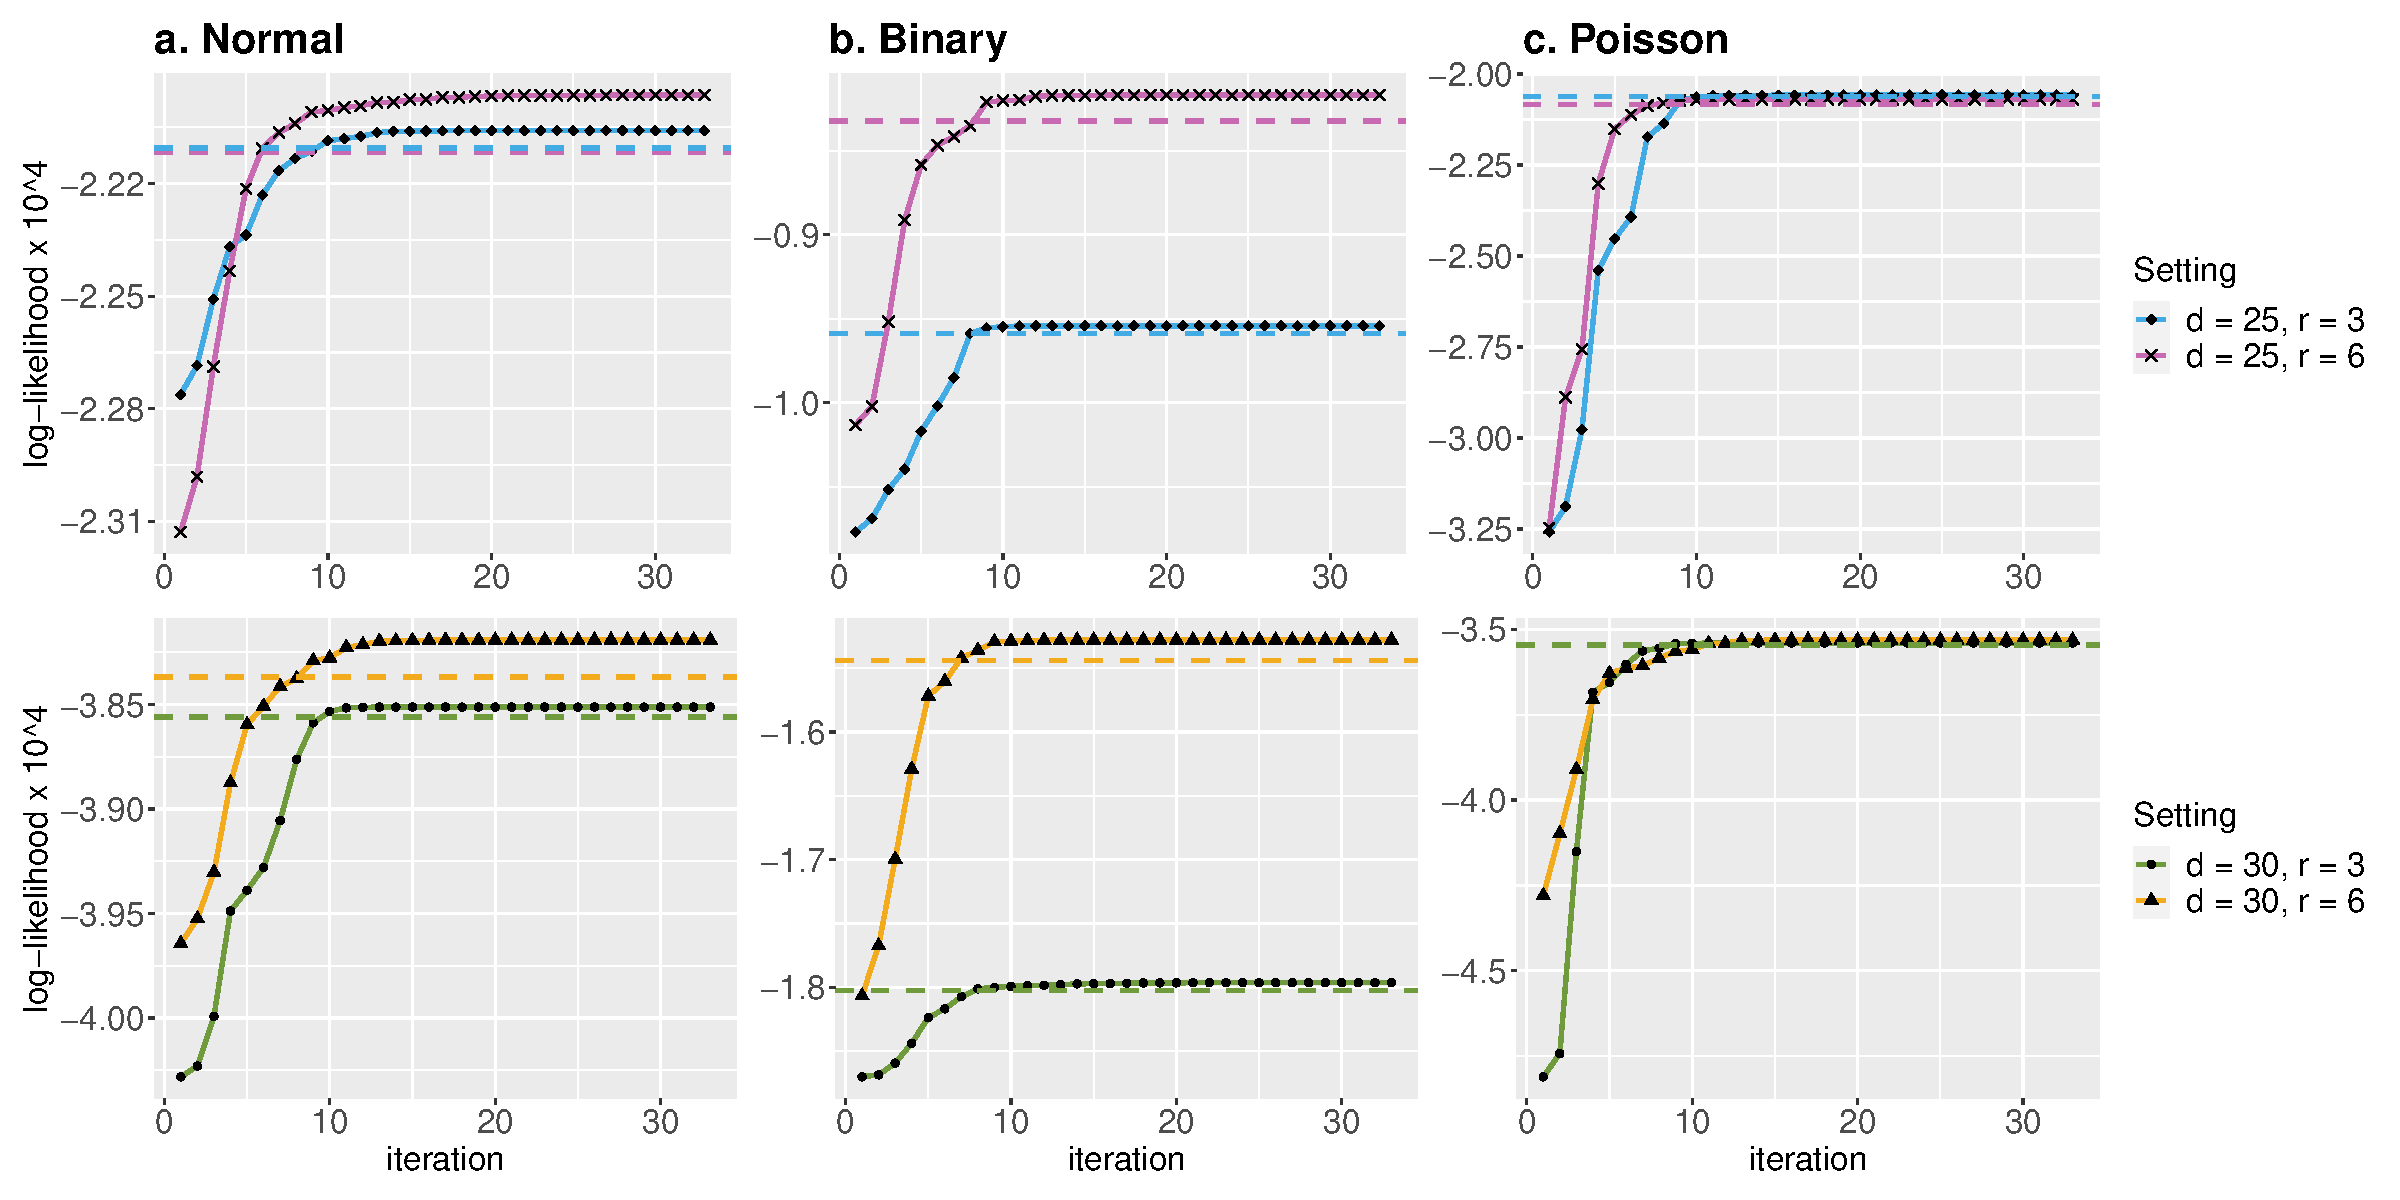
\includegraphics[width=15cm]{new_log.pdf}
\caption{Trajectory of the objective function with various dimension $d$ and rank $r$ under (a) Gaussian (b) Bernoulli (c) Poisson models. The dashed line represents the objective value at true parameter $\tL_{\tY}(\tB_{true})$. A micro-iteration refers to the update for one of the $K$ blocks. Four micro-iterations consist of a complete ``while'' iteration in Algorithm~\ref{alg:B}.}\label{fig:loglike}
\end{figure}



\subsection{Rank selection and time complexity}\label{sec:tuning}
Algorithm~\ref{alg:B} takes the rank $\mr$ as an input. Estimating an appropriate rank given the data is of practical importance. We propose to use Bayesian information criterion (BIC) and choose the rank that minimizes BIC; i.e.
\begin{align}\label{eq:BIC}
\hat \mr&=\argmin_{\mr=(r_1,\ldots,r_K)} \text{BIC}(\mr)\\
&=\argmin_{\mr=(r_1,\ldots,r_K)}\left[-2\tL_{\tY}(\hat \tB)+p_e(\mr)\log \left(\prod_k d_k\right) \right],
\end{align}
where $p_e(\mr)\stackrel{\text{def}}{=}\sum_k (p_k-r_k-1)r_k+\prod_k r_k$ is the effective number of parameters in the model. We choose $\hat \mr$ that minimizes $\text{BIC}(\mr)$ via grid search. Our choice of BIC aims to balance between the goodness-of-fit for the data and the degree of freedom in the population model. We test its empirical performance in Section~\ref{sec:simulation}.  

The computational complexity of our alternating optimization algorithm is $O\left(d \sum_k p^3_k\right)$ for each loop of iterations, where $d=\prod_k d_k$ is the total size of the response tensor. More precisely, the update of core tensor costs $O(r^3d)$, where $r=\prod_k r_k$ is the total size of the core tensor. The update of each factor matrix $\mM_k$ involves a GLM with a $d$-length response, and $d$-by-$(r_kp_k)$ feature matrix. Solving such a GLM requires $O(dr^3_kp^3_k)$, and therefore the cost for updating $K$ factors in total is $O( d\sum_k r^3_k p_k^3)$.



\subsection{Statistical properties}\label{subsec:statprob}
We assess the estimation accuracy using the deviation in the Frobenius norm. \fixme{Miaoyan}{needs revision...} For the true coefficient tensor $\trueB$ and its estimator $\hat \tB$, define
\[
\text{Loss}(\trueB,\ \hat \tB)=\FnormSize{}{\trueB- \hat \tB}^2.
\]

In modern applications, the response tensor and features are often large-scale. We are particularly interested in the high-dimensional region in which both $d_k$ and $p_k$ diverge; i.e.\ $d_k\to \infty$ and $p_k\to\infty$, while ${p_k\over d_k} \to \gamma_k \in[0,1)$. As the size of problem grows, and so does the number of unknown parameters. As such, the classical MLE theory does not directly apply. We leverage the recent development in random tensor theory and high-dimensional statistics to establish the error bounds of the estimation. 

  
  
\begin{assumption}\label{ass}We make the following assumptions:
\begin{enumerate}
\item [A1.] There exist two positive constants $c_1, c_2>0$ such that $c_1\leq \sigma_{\min}(\mX_k)\leq  \sigma_{\max}(\mX_k)\leq c_2$ for all $k\in[K]$. Here $\sigma_{\text{min}}(\cdot)$ and $\sigma_{\text{max}}(\cdot)$ denotes the smallest and largest singular values, respectively.
\item [A2.] There exist two positive constants $L,\ U>0$ such that $L\phi \leq \text{Var}(y_{i_1,\ldots,i_K}|\theta_{i_1,\ldots,i_K})\leq U\phi $ for all $|\theta_{i_1,\ldots,i_K}|\leq \alpha$.
\item[A2'.] Equivalently, there exists two positive constants $L,\ U>0$ such that $L\leq b''(\theta) \leq U$ for all $|\theta|\leq \alpha$, where $\alpha$ is the upper bound of the linear predictor. 

\end{enumerate}
\end{assumption}
The assumptions are fairly mild. Assumption A1 guarantees the non-singularity of the feature matrices, and Assumption A2 ensures the log-likelihood $\tY(\Theta)$ is strictly concave in the linear predictor $\Theta$. Assumption A2 and A2' are equivalent, because $\text{Var}(y_{i_1,\ldots,i_K}|\tX,\tB)=\phi b''(\theta_{i_1,\ldots,i_K})$ when $y_{i_1,\ldots,i_K}$ belongs to an exponential family~\citep{mccullagh1989generalized}. 

  
\begin{thm}[Statistical convergence]\label{thm:main}
Consider an order-$K$ dimensional-$(d_1,\ldots,d_K)$ tensor $\tY$ and multiple feature matrices $\mX_k\in\mathbb{R}^{d_k\times p_k}$, for $k\in[K]$. Suppose that, conditional on the features, the entries in $\tY$ are independent realizations from an exponential family distribution with conditional mean model~\eqref{eq:decomp}. Let $r_\text{total}=\prod_k r_k$, $r_{\max}=\max_k r_k$, and $\sigma_{\min}(\mM_k)$ be the smallest singular value of $\mM_k$. Assume that $\sigma_{\min}(\mM_k)>0$ and $\FnormSize{}{\mX_k} \asymp \Omega(\sqrt{d_k})$ as $d_k\to\infty$, for all $k\in[K]$. Under Assumption~\ref{ass}, there exist two constants $C_1, C_2>0$, such that, with probability at least $1-\exp(-C_1\sum_k p_k)$, 
\begin{equation}\label{eq:bound}
\textup{sin}^2 \Theta(\mM_k,\ \hat \mM_k) \leq  \frac{ C_{2}r_{\textup{total}}}{ r_{\max}\sigma^2_{\min}(\mM_k)}\frac{\sum_k p_k}{\prod_k d_k}, \quad\text{for all }k\in[K],
\end{equation}
and
\[
\FnormSize{}{\trueB- \hat \tB}^2\leq \frac{ C_{2} r_{\textup{total}}}{r_{\max}}\frac{\sum_k p_k}{\prod_k d_k}.
\]
Here, $C_2=C_2(\mr,\alpha, K)>0$ is a constant independent of the dimensions $\{d_k\}$ and $\{p_k\}$. 
\end{thm}

Theorem~\ref{thm:main} establishes the statistical convergence for the estimator~\eqref{eq:MLE}. Actually, the proof in section~\ref{sec:appedix} shows that the statistically optimal rate holds, not only for the MLE~\eqref{eq:MLE}, but also any local estimators $\hat \tB$ in the level set $\{\hat \tB \in \tP \colon \tL_{\tY} (\hat \tB) \geq \tL_{\tY} (\tB_{true}) \}$ satisfies the upper bound~\ref{thm:main}\fixme{Miaoyan}{Wrong statement based on current proof}. In Section~\ref{subsec:alg}, we implement empirical studies to verify the algorithmic stability to find a local optimum.


To gain further insight on the bound~\eqref{eq:bound}, we consider a special case when tensor dimensions are equal at each of the modes, i.e., $d_k=d$, $p_k=\gamma d$, $\gamma\in [0,1)$ for all $k\in[K]$, and the feature matrices $\mX_k$ are Gaussian design with i.i.d.\ $N(0,1)$ entries. To put the context in the framework of Theorem~\ref{thm:main}, we rescale the feature matrices into $\check \mX_k={1\over \sqrt{d}}\mX_k$ so that the singular values of $\check \mX_k$ are bounded by $1\pm \sqrt{\gamma}$. The result in~\eqref{eq:bound} implies that the estimated coefficient has a convergence rate $\tO({p\over d^K})$ in the scale of the original feature $\{\mX_k\}$. Therefore, our estimation is consistent as the dimension grows, and the convergence becomes especially favorably as the order of tensor data increases. 

As immediate applications, we obtain the convergence rate for the three examples mentioned in Section~\ref{sec:model}. Without loss of generality, we assume that the singular values of the $d_k$-by-$p_k$ feature matrix $\mX_k$ are bounded by $\sqrt{d_k}$. 


\begin{example}[Spatio-temporal growth model] The estimated type-by-time-by-space coefficient tensor converges at the rate $\tO\left({p+r+s\over dmn}\right)$ where $p\leq d$, $r\leq m$ and $s\leq n$. The estimation achieves consistency as long as the dimension grows in either of the three modes.
\end{example}

\begin{example} [Network population model] The estimated node-by-node-by-feature tensor converges at the rate $\tO\left({2d+p\over d^2n}\right)$ where $p\leq n$. The estimation achieves consistency as the number of individuals or the number of nodes grows. 
\end{example}

\begin{example} [Dyadic data with node attributes] The estimated feature-by-feature matrix converges at the rate $\tO\left({p\over d^2}\right)$ where $p\leq d$. Again, our estimation achieves consistency as the number of nodes grows. 
\end{example}

We conclude this section by providing the prediction accuracy, measured in KL divergence, for the response distribution.   

\begin{thm}[Prediction error]\label{thm:KL}
Assume the same set-up as in Theorem~\ref{thm:main}. Let $\mathbb{P}_{\tY_{\text{true}}}$ and $\mathbb{P}_{\hat \tY}$ denote the distributions of $\tY$ given the true parameter $\trueB$ and estimated parameter $\hat \tB$, respectively. Then, we have, with probability at least $1-\exp(C_1\sum_k p_k)$,
\[
\text{KL}(\mathbb{P}_{\tY_{\text{true}}},\ \mathbb{P}_{\hat \tY})\leq \frac{ C_{4}r_{\textup{total}}}{r_{\max}} {\sum_k p_k\over \prod_k d_k},
\]
where $C_4=C_4(\mr,\alpha, K)>0$ is a constant that independent of dimensions $\{d_k\}$ and $\{p_k\}$.
\end{thm}

\section{Numerical experiments}\label{sec:simulation}
We evaluate the empirical performance of our generalized tensor regression through simulations. We consider order-3 tensors with a range of distribution types. 
Unless otherwise specified, the conditional mean tensor is generated form model~\eqref{eq:decomp}, where the core tensor entries are i.i.d.\ drawn from Uniform[-1,1], the factor matrix $\mM_k$ is uniformly sampled (with respect to Haar measure) from matrices with orthonormal columns, and the feature matrix $\mX_k$ is either an identity matrix (i.e.\ no feature available) or Gaussian random matrix with i.i.d.\ entries from $N(0,\sigma_k^2)$. We set $\sigma_k=d_k^{-1/2}$ to ensure the singular values of $\mX_k$ are bounded as $d_k$ increases. The linear predictor $\Theta=\tC\times\{\mM_1\mX_1,\ldots,\mM_3\mX_3\}$ is scaled such that $\mnormSize{}{\Theta}=1$. Conditional on the linear predictor $\Theta=\entry{\theta_{ijk}}$, the entries in the tensor $\tY=\entry{y_{ijk}}$ are drawn independently according to one of the following three probabilistic models:

\begin{enumerate}
\item[(a)] (Gaussian). Continuous data $y_{ijk}\sim N\left(\alpha \theta_{ijk}, 1\right)$, for all $(i,j,k)\in[d_1]\times[d_2]\times[d_3]$.
\item[(b)] (Poisson). Count data $y_{ijk}\sim\text{Poi}\left( e^{\alpha \theta_{ijk}}\right)$, for all $(i,j,k)\in[d_1]\times[d_2]\times[d_3]$.
\item[(c)] (Bernoulli). Binary data $y_{ijk}\sim \text{Ber}\left( {e^{\alpha \theta_{ijk}} \over 1+e^{\alpha \theta_{ijk}}}\right)$, for all $(i,j,k)\in[d_1]\times[d_2]\times[d_3]$.
\end{enumerate}
Here $\alpha>0$ is a scalar controlling the magnitude of the effect size. In each simulation study, we report the mean squared error (MSE) for the coefficient tensor averaged across $n_{\text{sim}}=20$ replications. 

\subsection{Finite-sample Performance}

The first experiment assesses the selection accuracy of our BIC criterion~\eqref{eq:BIC}. We consider the balanced situation where $d_k=d$, $p_k=0.4d_k$ for $k=1,2,3$. We set $\alpha=4$ and consider various combinations of dimension $d$ and rank $\mr=(r_1,r_2,r_3)$. For each combination, we simulate tensor data following Gaussian and Poisson models. We then minimize BIC using a grid search over three dimensions. The hyper-parameter $\alpha$ is set to infinity in the fitting, which essentially imposes no prior on the coefficient magnitude. Table~\ref{tab:rank} reports the selected rank averaged over $n_{\text{sim}}=20$ replicates for Gaussian and Poisson models. We found that when $d=20$, the selected rank is slightly smaller than the true rank, and the accuracy improves immediately when the dimension increases to $d=40$. This agrees with our expectation, as in tensor regression, the sample size is related to the number of entries. A larger $d$ implies a larger sample size, so the BIC selection becomes more accurate. 


\begin{table}[tb]
\centering
\begin{tabular}{|c|cc|cc|}
\hline
True Rank &\multicolumn{2}{c|}{Dimension (Gaussian tensors)}&\multicolumn{2}{c|}{Dimension (Poisson tensors)}\\
$\mr$& $d=20$  &$d=40$&$d=20$ &$d=40$\\
\hline
$(3,\ 3,\ 3)$&$({\bf 3},\ 3,\ {\bf 3})$&$({\bf 3},\ {\bf 3},\ {\bf 3})$&$(2.0,\ 2.2,\ 2.1)$&$({\bf 3},\ {\bf 3},\ {\bf 3})$\\
$(4,\ 4,\ 6)$&$(3,\ 3,\ {\bf 6})$&$({\bf 4},\ {\bf 4},\ 5)$&$({\bf 4.0},\ {\bf 4.0},\ 5.2)$&$({\bf 4},\ {\bf 4},\ {\bf 6})$\\
$(6,\ 8,\ 8)$&$(5,\ 7,\ 7)$&$({\bf 6},\ {\bf 8},\ {\bf 8})$&$(5.0,\ 6.1,\ 7.1)$&$({\bf 6},\ {\bf 8},\ {\bf 8})$\\
\hline
\end{tabular}
\caption{Rank selection via BIC. Bold number indicates no significant difference between the estimate and the ground truth, based on a $z$-test with a level 0.05.}\label{tab:rank}
\end{table}


The second experiment evaluates the accuracy when features are available on all modes. We set $\alpha=10, d_k=d, p_k=0.4d_k, r_k=r\in\{2,4,6\}$ and increase $d$ from 30 to 60. Our theoretical analysis suggests that $\hat \tB$ has a convergence rate $\tO(d^{-2})$ in this setting. Figure~1 plots the estimation error versus the ``effective sample size'', $d^2$, under three different distribution models. We found that the empirical MSE decreases roughly at the rate of $1/d^2$, which is consistent with our theoretical ascertainment. We also observed that, tensors with higher ranks tend to yield higher estimation errors, as reflected by the upward shift of the curves as $r$ increases. Indeed, a larger $r$ implies a higher model complexity and thus greater difficulty in the estimation. Similar behaviors can be observed in the non-Gaussian data in Figure~\ref{fig:dim}b-c. 

\begin{figure}[t]
\centering
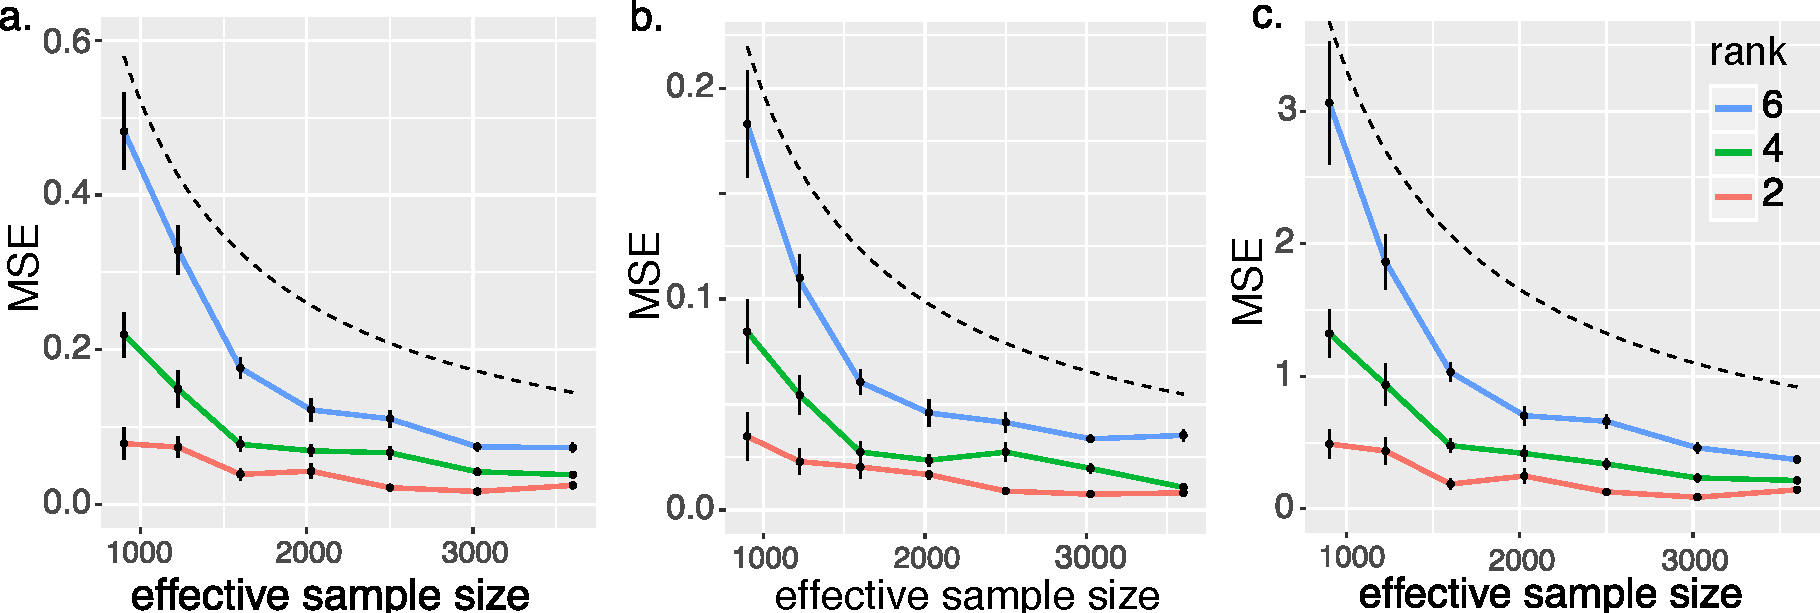
\includegraphics[width=15cm]{dimension.pdf}
\caption{Estimation error against effective sample size. The three panels depict the MSE when the response tensors are generated form (a) Gaussian (b) Poisson and (c) Bernoulli models. The dashed curves correspond to $\tO({1/d^2})$.}\label{fig:dim}
\end{figure}

The third experiment investigates our model's ability in handling correlation among coefficients. We mimic the scenario of brain imaging analysis. A sample of $d_3=50$ networks are simulated, one for each individual. Each network measures the connections between $d_1=d_2=20$ brain nodes. We simulate $p=5$ features for the each of the 50 individuals. These features may represent, for example, age, gender, cognitive score, etc. Recent study~\citep{robinson2015dynamic} has suggested that brain connectivity networks often exhibit community structure represented as a collection of subnetworks, and each subnetwork is comprised of a set of spatially distributed brain nodes. To accommodate this structure, we utilize the stochastic block model~\citep{abbe2017community} to generate the effect size. Specifically, we partition the nodes into $r$ blocks by assigning each node to a block with uniform probability. Edges within a same block are assumed to share the same feature effects, where the effects are drawn i.i.d.\ from $N(0,1)$. We then apply our tensor regression model to the network data using the BIC-selected rank. Note that in this case, the true model rank is unknown; the rank of a $r$-block matrix is not necessarily equal to~$r$~\citep{zeng2019multiway}. 

\begin{figure}[tb]
\centering
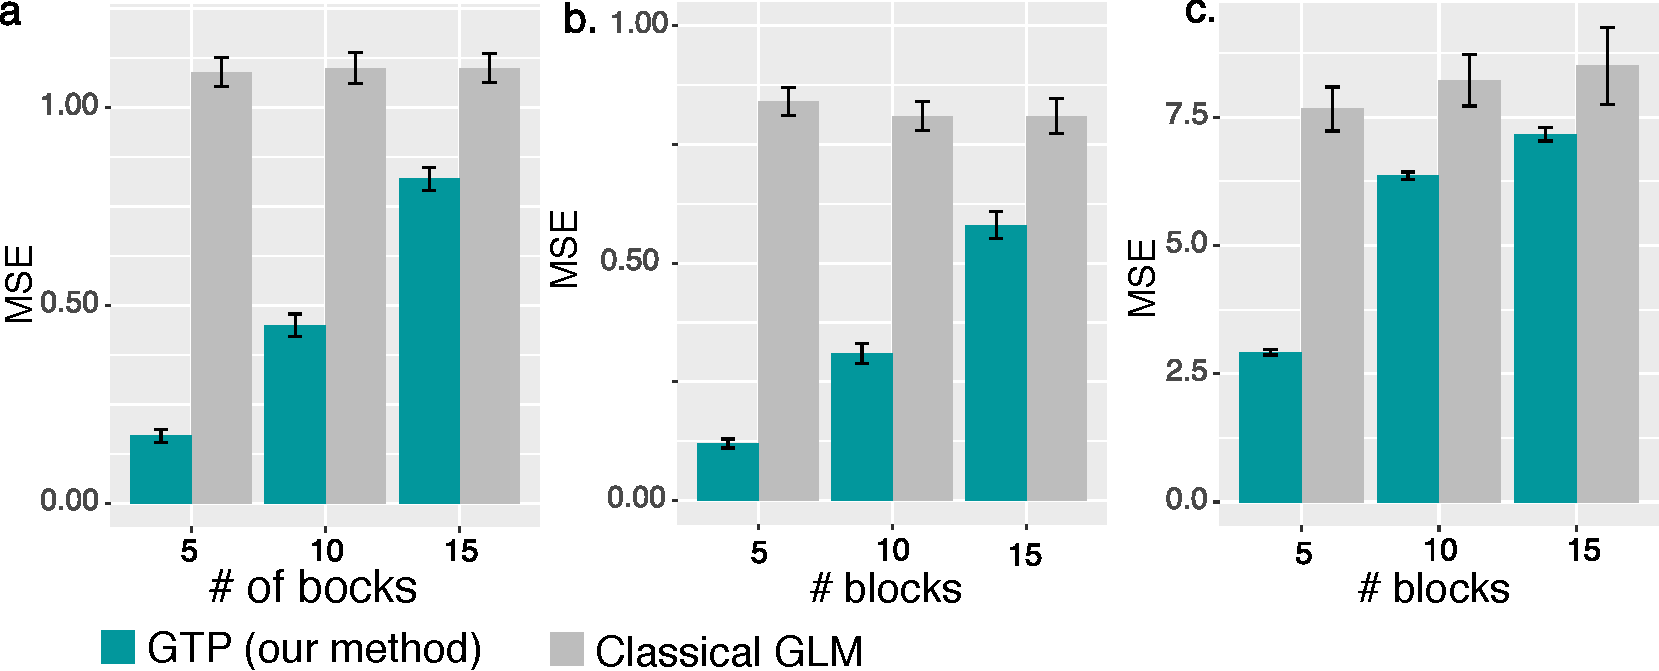
\includegraphics[width=15cm]{comparison.pdf}
\caption{Performance comparison when the networks have block structure. The three panels depict the MSE when the response tensors are generated form (a) Gaussian (b) Poisson and (c) Bernoulli models. The $x$-axis represents the number of blocks in the networks. }\label{fig:glm}
\end{figure}


Figure~\ref{fig:glm} compares the MSE of our method with a classical GLM approach. A classical GLM is to regress the dyadic edges, one at a time, on the features, and this model is repeatedly fitted for each edge. As we find in Figure~\ref{fig:glm}, out tensor regression method achieves significant error reduction in all three models considered. The outer-performance is significant in the presence of large communities, and even in the less structured case ($\sim 20/15=1.33$ nodes per block), our method still outer-performs GLM. The possible reason is that the massive GLM approach does not account for the correlation among the edges, and suffer from overfitting. In contrast, the low-rankness in our modeling automatically identifies the shared information across entries. By selecting the rank in a data-driven way, our method is able to achieve accurate estimation with improved interpretability. 

\subsection{Comparison with alternative methods}
We compare our generalized tensor regression ({\bf GTR}) with three other supervised tensor methods:
\begin{itemize}
\item  Higher-order low-rank regression ({\bf HOLRR},~\citep{rabusseau2016low}) is a least-square based tensor regression that allows features on a single mode. 
\item Higher-order partial least square ({\bf HOPLS},~\citep{zhao2012higher}) is a dimension-reduction method that jointly models a tensor response and a tensor feature. 
\item Subsampled tensor projected gradient ({\bf TPG},~\citep{yu2016learning}) tackles the same question as {\bf HOLRR} but instead uses a different algorithm to solve the problem. 
\end{itemize}
These three methods are the closest algorithms to ours, in that they relate a tensor response to features using a low-rank structure. All the three methods allow only Gaussian data, whereas ours is applicable to any exponential family distribution including Gaussian, Bernoulli, Multinomial, etc. For fair comparison, we consider only Gaussian response in the simulation. We measure the accuracy using mean squared prediction error, $\text{MSPE}=\sqrt{\sum_kd_k}\FnormSize{}{\hat \tY-\mathbb{E}(\tY|\tX)}$, where $\hat \tY$ is the fitted value from each of the methods. 

The comparison was assessed from three aspects: (a) benefit of incorporating features from multiple modes; (b) prediction error with respect to sample size; (c) sensitivity of accuracy with respect to model complexity. We use similar simulation setups as in our experiment II, but consider combinations of rank ($\mr=(3,3,3)$ vs.\ $(4,5,6)$), noise ($\sigma = 1/2$ vs. $1/4$), and dimension ($d$ ranging from 20 to 100 for modes with features, $d = 20$ for modes without features). 

Figure~\ref{fig:compare} shows the averaged prediction error across 20 replicates. We see that our {\bf GTR} outperforms others, especially in the high-rank high-noise setting. As the number of informative modes (i.e. modes with available features) increases, the {\bf GTR} exhibits a reduction in error whereas others have increased errors. This showcases the benefit toward prediction via incorporation of interactive features. Note that our method {\bf GTR} is most comparable to {\bf HOLRR} when there is only a single informative mode. In such a case, both methods share a same cost function but have different algorithms. {\bf GTR} alternates between informative and non-informative modes, whereas {\bf HOLRR} approximates the non-informative modes via unfolded response alone. The accuracy gain in Figure~\ref{fig:compare} demonstrates the benefit of alternating algorithm -- having informative modes also improves the estimation along non-informative modes. 

\begin{figure}[ht]
\centering
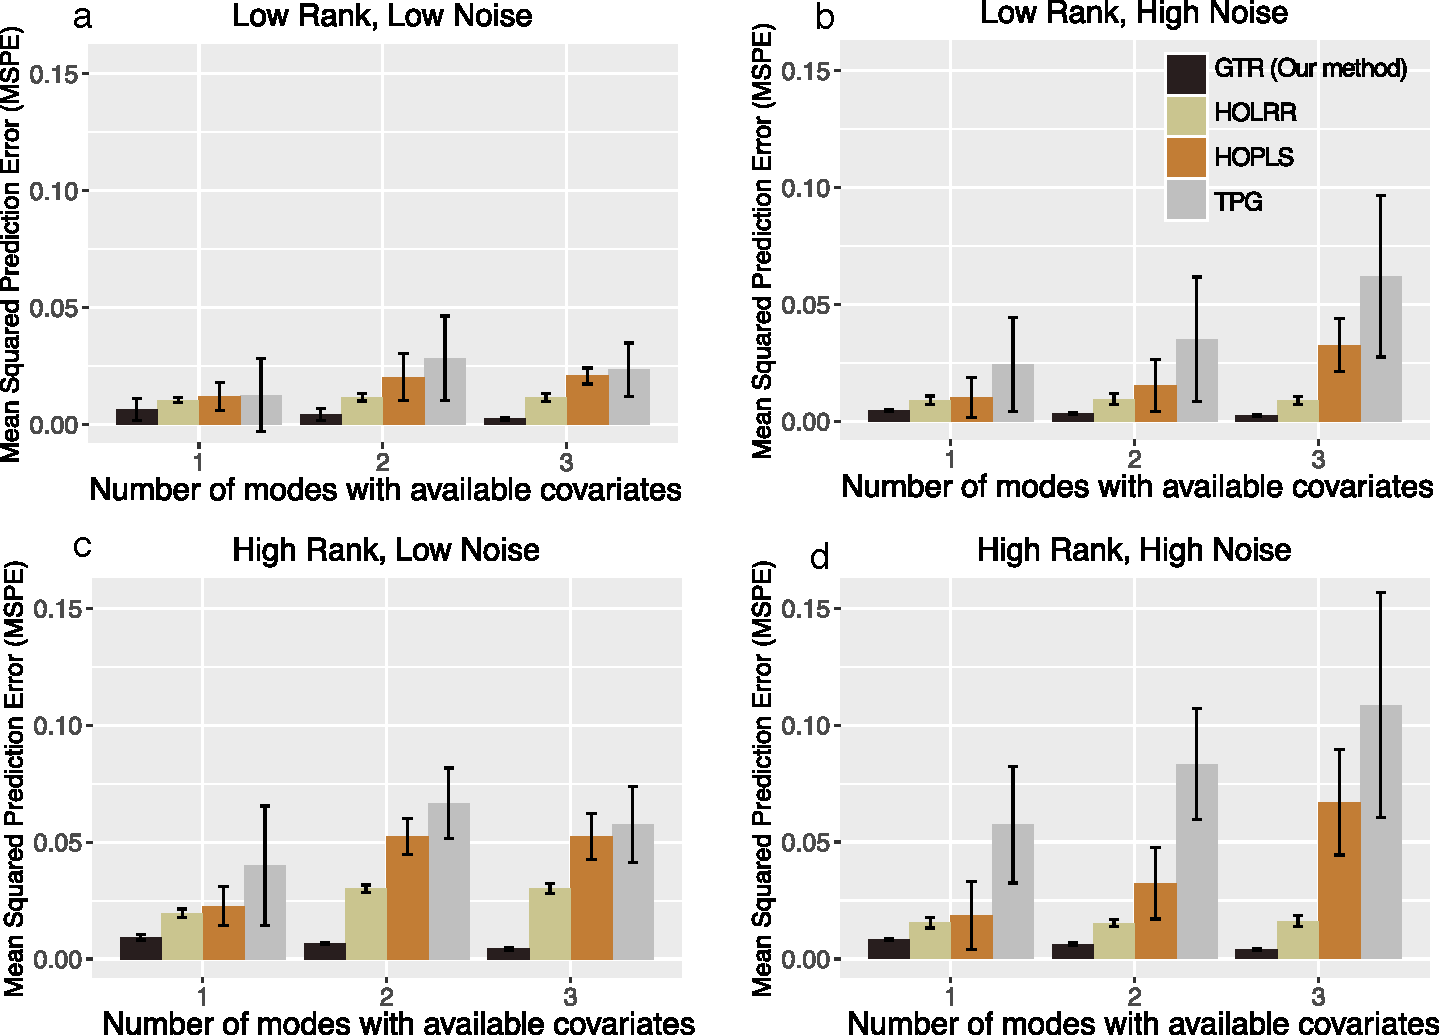
\includegraphics[width=12cm]{merge.pdf} 

\caption{Comparison of MSPE versus the number of modes with features. We consider rank $\mr=(3,3,3)$ (low), $\mr=(4,5,6)$ (high), and noise $\sigma=1/2$ (high), $\sigma=1/4$ (low).}~\label{fig:compare}

\end{figure}


Figure~\ref{fig:compare2} compares the prediction error with respect to sample size. The sample size is the total number of entries in the tensor. In the low-rank setting, our method has similar performance as {\bf HOLRR}, and the improvement becomes more pronounced when the rank increases. Neither {\bf HOPLS} nor {\bf TPG} has satisfactory performance in high-rank or high-noise settings. One possible reason is that a higher rank implies a higher inter-mode complexity, and our {\bf GTR} method lends itself well to this context. 


\begin{figure}[ht]
\centering
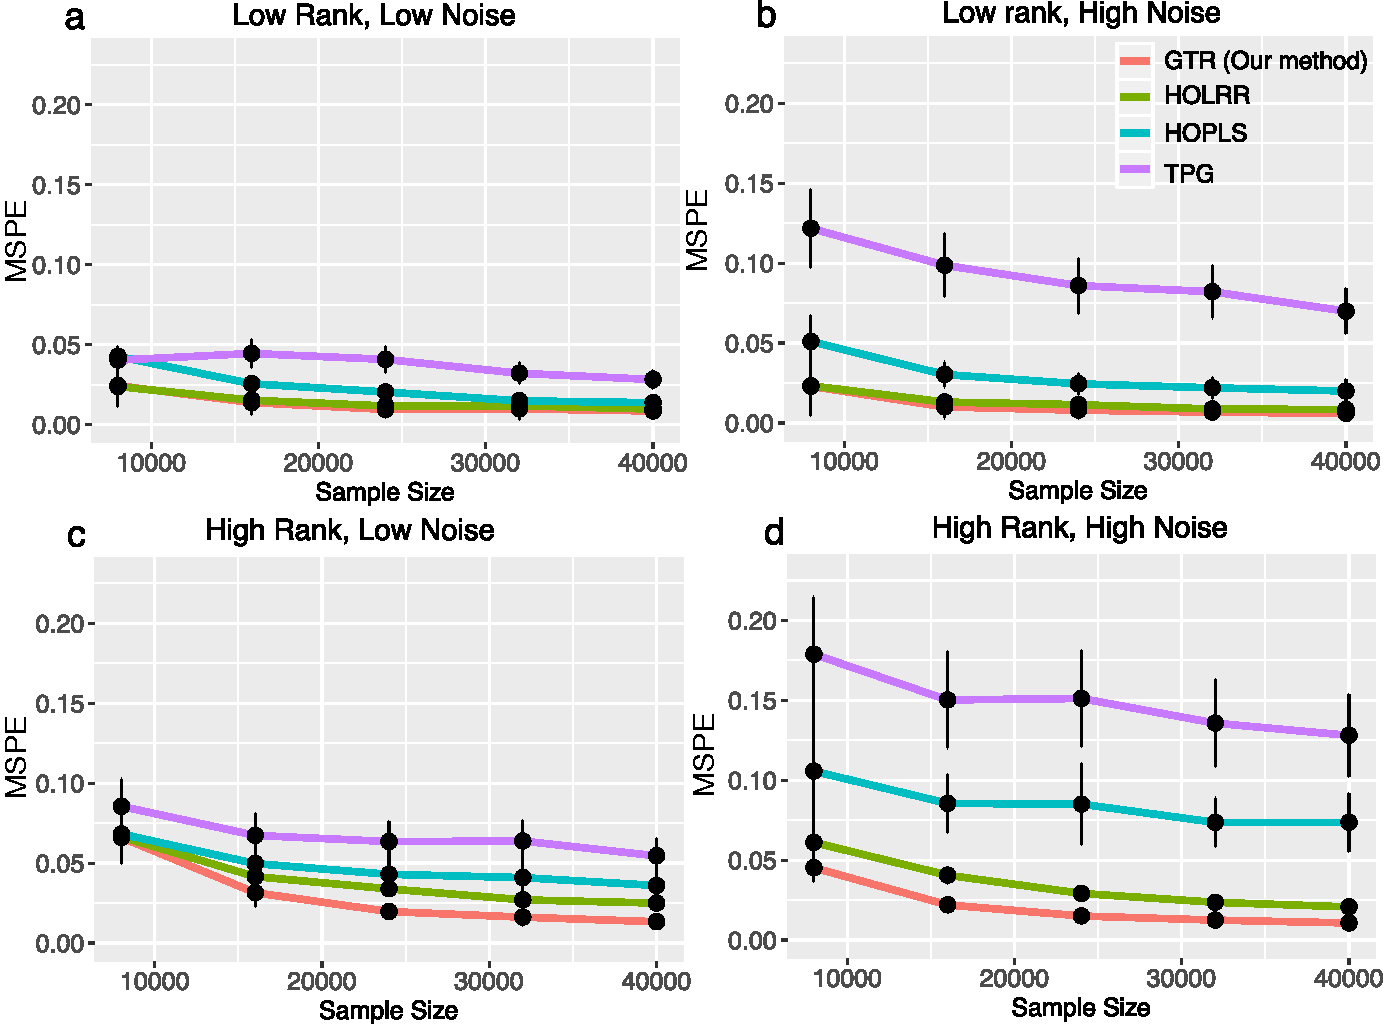
\includegraphics[width=12cm]{merge2.pdf} 

\caption{Comparison of MSPE versus sample size. We consider rank $\mr=(3,3,3)$ (low), $\mr=(4,5,6)$ (high), and noise $\sigma=1/2$ (high), $\sigma=1/4$ (low). }~\label{fig:compare2}

\end{figure}

\section{Data analyses}\label{sec:data}
We apply our tensor regression model to two datasets. The first application concerns the brain network modeling in response to individual attributes (i.e.\ feature on one mode), and the second application focuses on multi-relational network analysis with dyadic attributes (i.e.\ features on two modes). 

\subsection{Analysis of human brain connection data}
The Human Connectome Project (HCP) aims to build a ``network map'' that characterizes the anatomical and functional connectivity within healthy human brains~\citep{HCP}. We take a subset of HCP data that consists of 136 brain structural networks, one for each individual. Each brain network is represented as a 68-by-68 binary matrix, where the entries encode the presence or absence of fiber connections between the 68 brain regions. We consider four individual features: gender (65 females vs.\ 71 males), age 22-25 ($n=35$), age 26-30 ($n=58$), and age 31+ ($n=43$). The goal is to identify the connection edges that are affected by the individual feature. A key challenge in brain network is that the edges are correlated; for example, two edges may stem out from a same brain region, and it is of importance to take into account the within-dyad dependence. 


\begin{figure}[H]
\centering

\includegraphics[width=13cm]{HCP.pdf}
\caption{Top edges with large effects. Red edges represent relatively strong connections and blue edges represent relatively weak connections. (a) Global effect; (b) Female effect; (c) Age 22-25; (d) Age 31+.}\label{fig:brain}
\end{figure}

We fit the tensor regression model to the HCP data. The response is a binary tensor $\tY\in\{0,1\}^{68\times 68\times 136}$ and the features are of dimension 4 along the 3$^{\text{rd}}$ mode. The BIC selection suggests a rank $\mr=(10,10,4)$ with log-likelihood $\tL_{\tY}=-174654.7$. Figure~\ref{fig:brain} shows the top edges with high effect size, overlaid on the Desikan atlas brain template~\citep{desikan2006automated,xia2013brainnet}. We utilize the sum-to-zero contrasts in the effects coding and depicted only the top 3\% edges whose connections are non-constant across the sample. It is observed that the global connection exhibits clear spatial separation, and that the nodes within each hemisphere are more densely connected with each other (Figure~\ref{fig:brain}a). In particular, the superior-temproal (\emph{SupT}), middle-temporal (\emph{MT}) and Insula are the top three popular nodes in the network. Interestingly, female brains display higher inter-hemispheric connectivity, especially in the frontal, parental and temporal lobes (Figure~\ref{fig:brain}b). This is in agreement with a recent study showing that female brains are optimized for inter-hemispheric communication~\citep{ingalhalikar2014sex}. We also found several edges with declined connection in the group Age 31+. Notably, those edges involve Frontal-pole (\emph{Fploe}), superior-frontal (\emph{SupF}) and Cuneus nodes. The Frontal-pole region has long been known for its importance in memory and cognition, and the detected decline with age further highlights its biological importance. 

Figure~\ref{fig:s1} compares the estimated coefficients from our method (tensor regression) with those from classical GLM approach. A classical GLM is to regress the brain edges, one at a time, on the individual-level features, and this logistic model is repeatedly fitted for every edge $\in [68]\times [68]$. As we can see in the figure, our tensor regression shrinkages the coefficients towards center, thereby enforcing the sharing between coefficient entries. 

\begin{figure}[H]
\centering
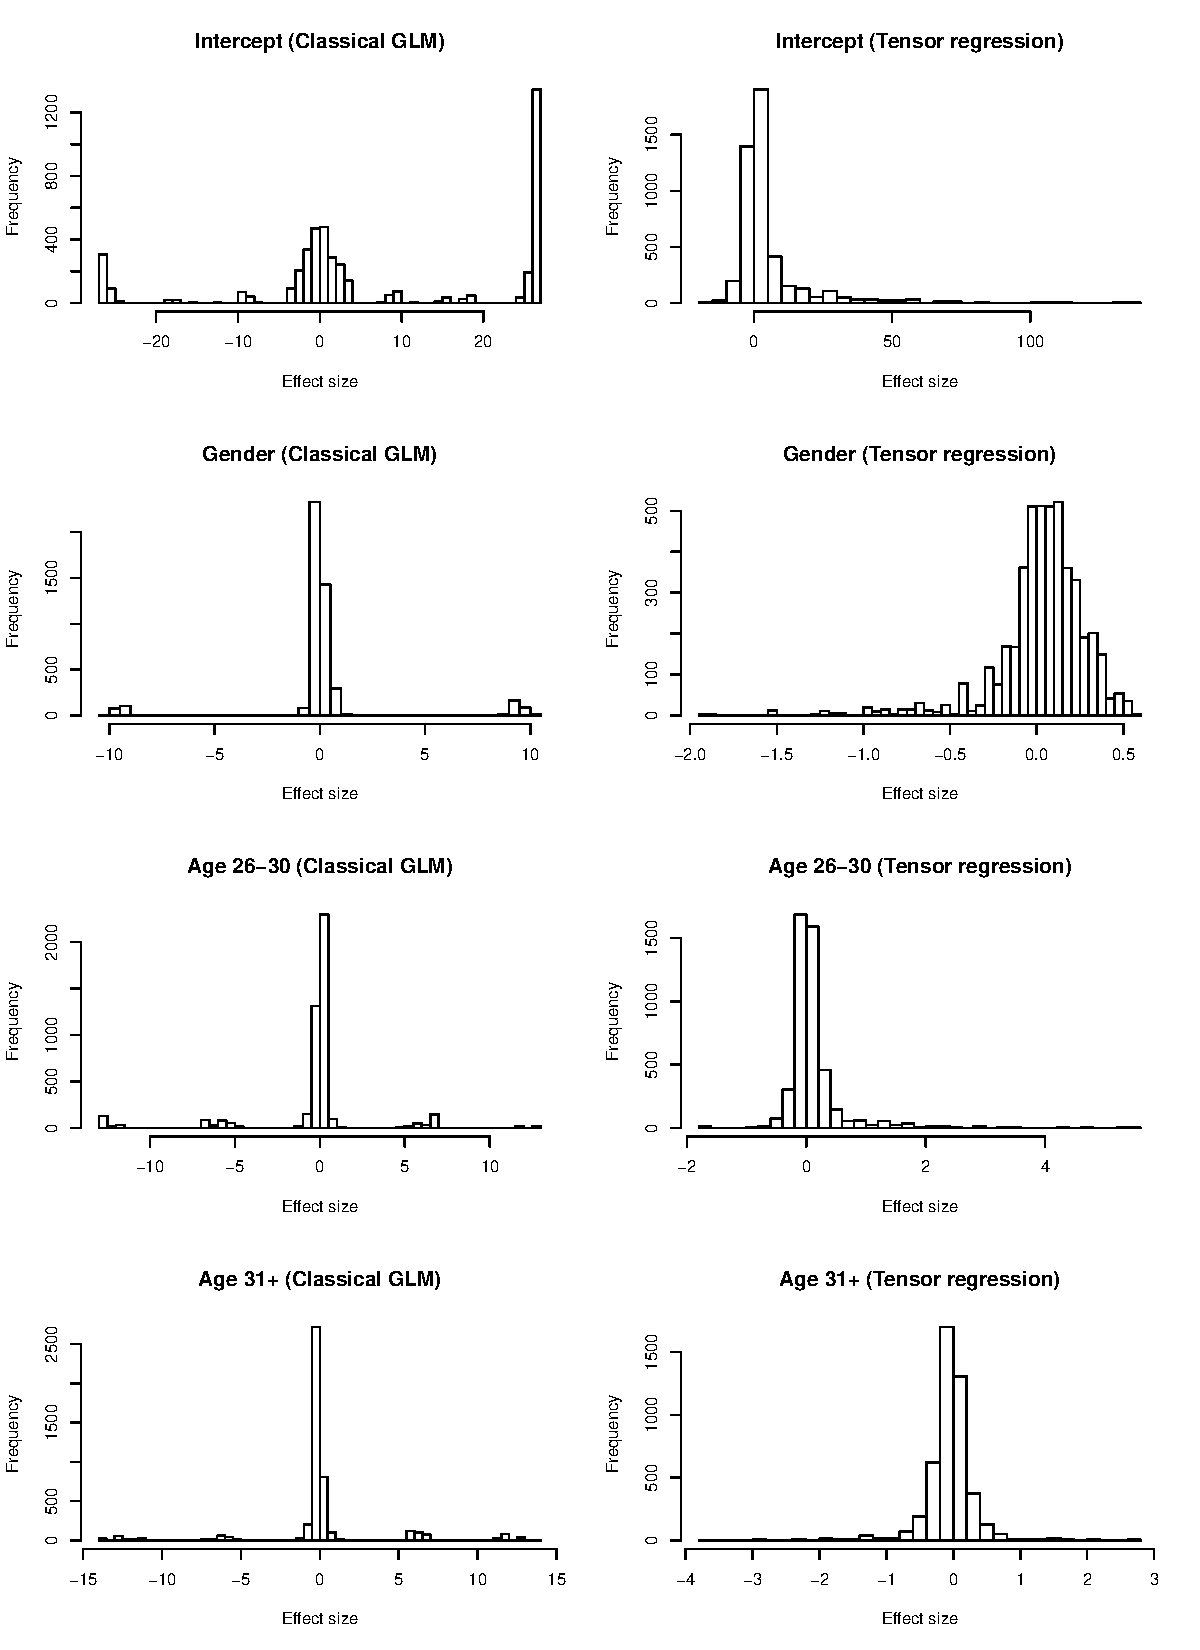
\includegraphics[width=16cm]{compare.pdf}
\caption{Comparison of coefficient estimation in the HCP data.}\label{fig:s1}
\end{figure}

\subsection{Analysis of political relational data}

The second application concerns the multi-relational network analysis with node-level attributes. We consider \emph{Nations} dataset~\citep{nickel2011three} which records 56 relations among 14 countries between 1950 and 1965. The multi-relational networks can be organized into a $14 \times 14 \times 56$ binary tensor, with each entry indicating the presence or absence of a connection, such as ``sending tourist to'', ``export'', ``import'', between countries. The 56 relations span the fields of politics, economics, military, religion, and so on. In addition, country-level attributes are also available, and we focus on the following six features: \emph{constitutional, catholics, lawngos, politicalleadership, geographyx}, and \emph{medicinengo}. The goal is to identify the variation in connections due to country-level attributes and interactions thereof. One of the key features is that the 56 relations are correlated, and we would like to take that into account in assessing the feature effects. 


We applied our tensor regression model to the \emph{Nations} data. The multi-relational network $\tY\in\{0,1\}^{14\times 14\times 56}$ was treated as the response tensor, and the country attributes $\mM\in\mathbb{R}^{14\times 6}$ were treated as features on both the 1st and 2nd modes. The BIC criterion suggests a rank $\mr=(4,4,4)$ for the coefficient tensor $\tB\in\mathbb{R}^{6\times 6 \times 56}$. Table~\sref{fig:s1} shows the $K$-mean clustering of the 56 relations based on the 3$^\text{rd}$ mode factor $\mM_3\in\mathbb{R}^{56\times 4}$. We found that the relations reflecting the similar aspects of international affairs are grouped together. In particular, Cluster I consists of political relations such as \emph{officialvisits, intergovorgs}, and \emph{militaryactions}; Clusters II and III capture the economical relations such as \emph{economicaid, booktranslations, tourism}; and Cluster IV represents the Cold War alliance blocs. The similarity among entities in each cluster suggests the plausibility of our dimension reduction. 


\begin{figure}[H]
\centering
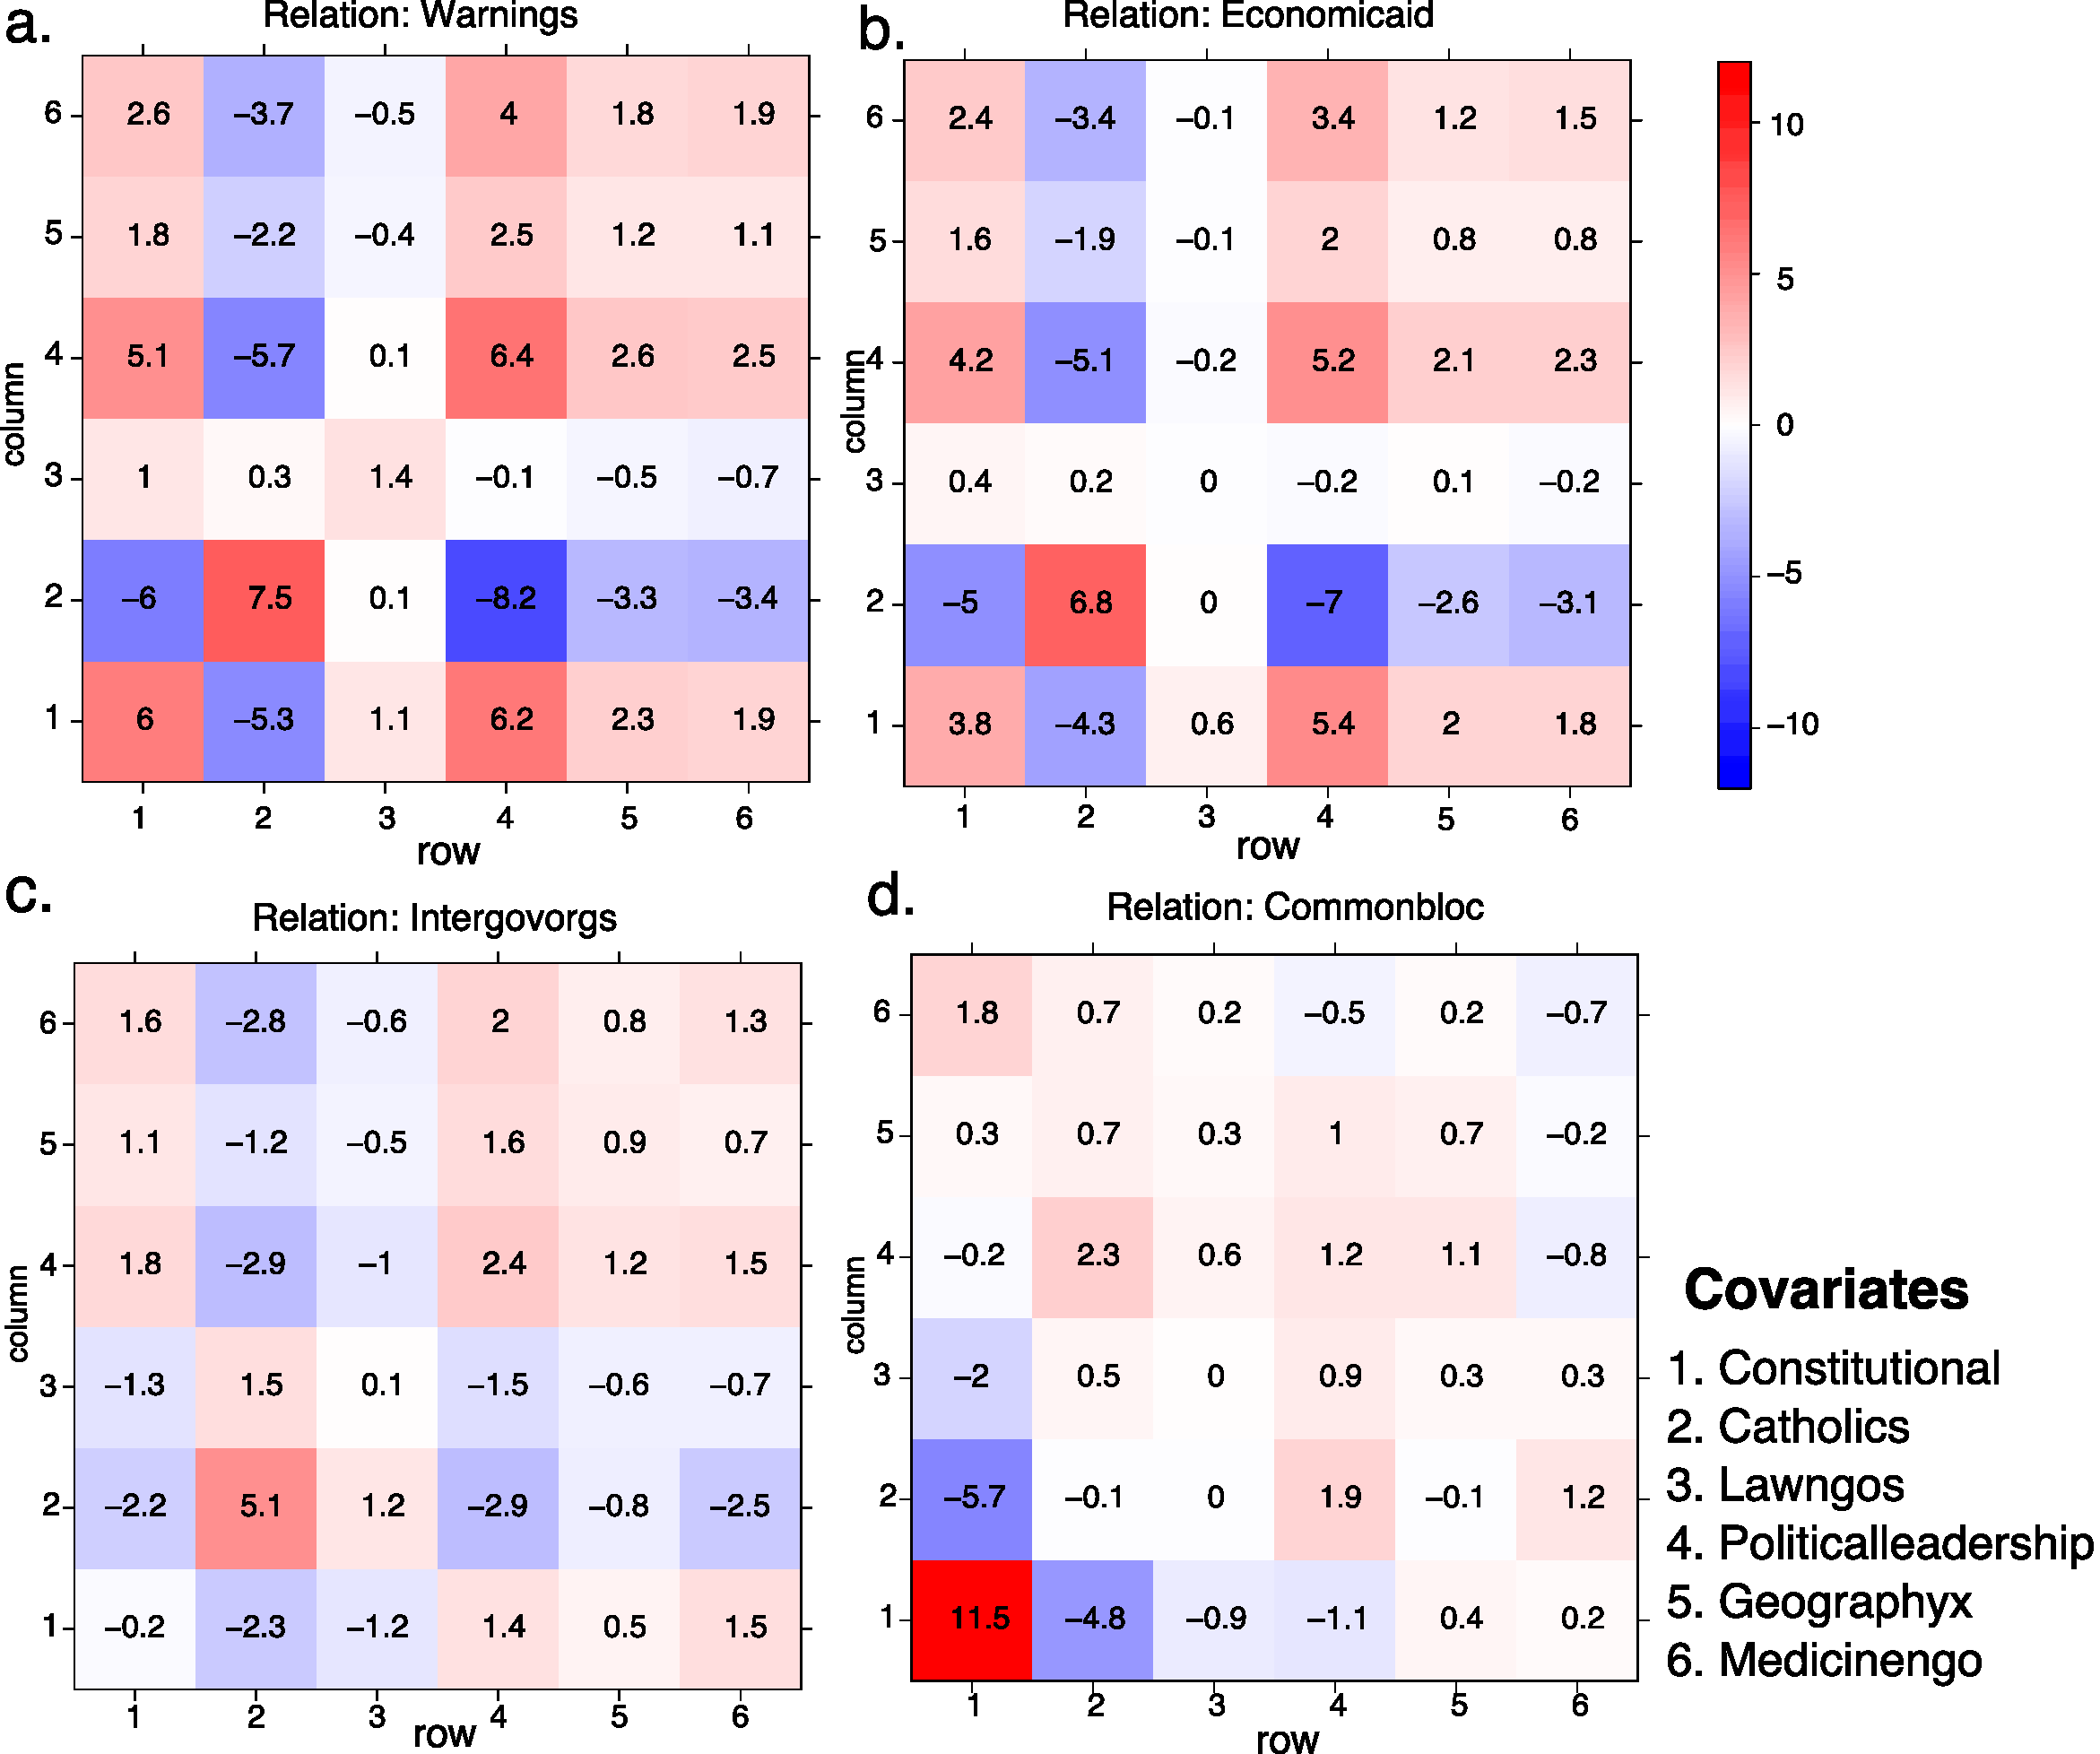
\includegraphics[width=14cm]{coef.pdf}
\caption{Effect estimation in the \emph{Nations} data. Panels (a)-(d) represent the estimated effects of country-level attributes towards the connection probability, for relations \emph{warnning}, \emph{economicaid},\emph{intergovorg}, and \emph{commonblock}, respectively. }\label{fig:est}
\end{figure}


\begin{table}[H]
\begin{tabular}{c|c|l}
\hline
\multirow{5}{*}{Cluster I}  & Government &officialvisits, intergovorgs,  militaryactions,  \\
&&negativebehavior, boycottembargo, aidenemy, negativecomm, \\
&&protestsunoffialacts,    nonviolentbehavior, emigrants,  \\
&&timesincewar, commonbloc2, rintergovorgs3, relintergovorgs\\
&&violentactions, duration,accusation,relexports\\
\hline
\multirow{6}{*}{Cluster II}& Economics &economicaid, booktranslations, tourism,  \\
&& conferences, severdiplomatic, expeldiplomats, attackembassy, \\
&& reltourism, tourism3, relemigrants, emigrants3, students, \\
&&exports, exports3, lostterritory, dependent, militaryalliance  \\
&&relbooktranslations, releconomicaid, unweightedunvote, \\
&& warning, relstudents,\\
\hline
\multirow{3}{*}{Cluster III} & treaties &treaties, reltreaties, exportbooks, relexportbooks,  \\
&&relngo, ngoorgs3, embassy, reldiplomacy, timesinceally, \\
&&independence, commonbloc1,weightedunvote, ngo,\\
\hline
Cluster IV & Politics &commonbloc0, blockpositionindex\\
\hline
\end{tabular}
\caption{$K$-means clustering of relations based on factor matrix in the coefficient tensor.}\label{tab:s1}
\end{table}


To investigate the effects of dyadic attributes towards connections, we depicted the estimated coefficients $\hat \tB=\entry{\hat b_{ijk}}$ for several relation types (Figure~\ref{fig:est}). Note that entries $\hat b_{ijk}$ can be interpreted as the contribution, at the logit scale, of feature pair $(i,j)$ ($i$th feature for the ``sender'' country and $j$th feature for the ``receiver'' country) towards the connection of relation $k$.  Several interesting findings emerge from the observation. We found that relations belonging to a same cluster tend to have similar feature effects. For example, the relations \emph{warnings} and \emph{ecnomicaid} are classified into Cluster II, and both exhibit similar feature pattern (Figure~\ref{fig:est}a-b). Moreover, the majority of the diagonal entries $\hat \tB(i,i,k)$ positively contribute to the connection. This suggests that countries with coherent attributes tend to interact more often than others. We also found that the \emph{constitutional} attribute is an important predictor for the \emph{commonbloc} relation, whereas the effect is weaker for other relations (Figure~\ref{fig:est}d). This is not surprising, as the block partition during Cold War is associated with the \emph{constitutional} attribute. 


\section{Conclusion}\label{sec:con}
\fixme{Miaoyan}{No more than 35 pages. Reserve at least 1.5 pages for Conclusion}
We have developed a generalized tensor regression with features on multiple modes. A fundamental feature of tensor-valued data is the statistical interdependence among entries. Our proposed rank-constrained estimation achieves high accuracy with sound theoretical guarantees. The estimation accuracy is quantified via deviation in the Frobenius norm and K-L divergence. Other measures of accuracy may also be desirable, such as the spectral norm or the maximum norm of the deviation. Exploiting the properties and benefits of different error quantification warrants future research.
 
 
 \fixme{Miaoyan}{Add two more paragraphs: 
 %Our method leverages on the alternating updating algorithm for the optimization. Although a non-convex optimization procedure such as Algorithm~\ref{alg:binary} has no guarantee on global optimality, our numerical experiments have suggested that, upon random initializations, the convergence point $\hat\Theta$ is often satisfactory, in that the corresponding objective value $\tL_{\tY}(\hat\Theta)$ is close to the objective value $\tL_{\tY}(\trueT)$. When starting from random initializations, there could be multiple estimates, whose objective values are all greater than $\tL_{\tY}(\trueT)$. In theory, any of those choices perform equally well in estimating $\trueT$. In this sense, local optimality is not necessarily a severe concern in our context. On the other hand, characterizing global optimality for non-convex optimization problem of this type is itself of great interest. There has been recent progress investigating the landscape of non-convex optimization involving tensors~\citep{anandkumar2014tensor, richard2014statistical, ge2017optimization}. The problem is challenging, as the geometry can  depend on multiple factors including the tensor rank, dimension, and factorization form. In some special cases such as rank-1 or orthogonally decomposable tensors, one may further obtain the required asymptotical number of initializations, however, at the cost of more stringent assumptions on the target tensor~\citep{anandkumar2014tensor, richard2014statistical}. We leave the pursuit of optimization landscape as future research.
%Another an.. is the (conditional) independence assumption on the tensor entries. Instead of glm, we may introduce a more general tensor-variate distribution on the $\tY$. For the case of normal distribution. For random effects.....
2. Assumption on (conditional) independence assumption on the tensor entries. Mixed effect model, tensor-variate normal distribution..Current approach is to use fixed factor; or a combination of fixed factor + random effects. 
3. Inference. ... uncertainly quantification... bootstrap ....  Testing for Interaction + main effects. 
}

\section*{Acknowledgements}
This research was supported by NSF grant DMS-1915978 and the University of Wisconsin-Madison, Office of the Vice Chancellor for Research and Graduate Education with funding from the Wisconsin Alumni Research Foundation. 
%The authors would like to thank Chen Zhang from Wisconsin State Lab of Hygiene for help with figure 4. 

\fixme{miaoyan}{references need update..}

\bibliography{tensor_wang}
\bibliographystyle{apalike}


\newpage
\begin{center}
{\large\bf SUPPLEMENTARY MATERIAL}
\end{center}

\appendix


\section{Proofs}\label{sec:appedix}
\begin{proof}[Proof of Theorem~\ref{thm:main}]
Define $\ell(\tB)=\mathbb{E}(\tL_{\tY}(\tB))$, where the expectation is taken with respect to $\tY\sim \trueB$ under the model with true parameter $\trueB$. We first prove the following two conclusions:
\begin{enumerate}
\item[C1.] There exists two positive constants $C_1$, $C_2>0$, such that, with probability at least $1-\exp(-C_1\log K\sum_k p_k)$, the stochastic deviation, $\tL_{\tY}(\tB)-\ell(\tB)$, satisfies
\[
|\tL_{\tY}(\tB)-\ell(\tB)|=|\langle \tE,\ \tB\times_1\mX_1\times_2\cdots\times_K \mX_K\rangle| \leq C_2\FnormSize{}{\tB} \sqrt{{\prod_k r_k \over \max_k r_k} \sum_k p_k}.
\]
\item[C2.] The inequality $\ell(\hat \tB) - \ell(\trueB) \leq  -{L\over 2}\FnormSize{}{\hat \Theta-\trueT}^2$ holds, where $L>0$ is the lower bound for $\min_{|\theta|\leq \alpha}|b''(\theta)|$. 
\end{enumerate}

To prove C1, we note that the stochastic deviation can be written as:
\begin{align}\label{bound}
\tL_{\tY}(\tB)-\ell(\tB)&=\langle \tY-\mathbb{E}(\tY|\tX),\ \Theta(\tB)\rangle\notag \\
&= \langle \tY- b'(\trueT),\ \Theta\rangle \notag \\
&= \langle \tE\times_1\mX^T_1\times_2\cdots\times_K\mX^T_K,\ \tB\rangle,
\end{align}
where $\tE\stackrel{\text{def}}{=}\tY-b'(\trueT)$, and the second line uses the property of exponential family that $\mathbb{E}(\tY|\tX)=b'(\trueT)$. Based on Proposition~\ref{prop}, the boundedness of $b''(\cdot)$ implies that $\tE$ is a sub-Gaussian-$(\phi U)$ tensor. Let $\check\tE\stackrel{\text{def}}{=}\tE\times_1\mX^T_1\times_2\cdots\times_K\mX^T_K$. By Proposition~\ref{prop:sub}, $\check \tE$ is a $(p_1,\ldots,p_K)$-dimensional sub-Gaussian tensor with parameter bounded by $C=\phi Uc^{K}_2$. Here $c_2>0$ is the upper bound of $\sigma_{\max}(\mX_k)$. Applying Cauchy-Schwarz inequality to~\eqref{bound} yields
\begin{equation}\label{eq:bound2}
|\tL_{\tY}(\tB)-\ell(\tB)|\leq \norm{\check \tE} \nnorm{\tB},
\end{equation}
where $\norm{\cdot}$ denotes the tensor spectral norm and $\nnorm{\cdot}$ denotes the tensor nuclear norm. The nuclear norm $\nnorm{\tB}$ is  bounded by $\nnorm{\tB}\leq \sqrt{{\prod_k r_k \over \max_k r_k}}\FnormSize{}{\tB}$ (c.f.~\citep{wang2018learning,wang2017operator}). The spectral norm $\norm{\check \tE}$ is bounded by $\norm{\check \tE}\leq C_2 \sqrt{\sum_k p_k}$ with probability at least $1-\exp(-C_1\log K \sum_kp_k)$ (c.f.~\citep{wang2018learning,tomioka2014spectral}). Combining these two bounds with~\eqref{eq:bound2}, we have, with probability at least $1-\exp(-C_1\log K \sum_kp_k)$, 
\[
|\tL_{\tY}(\tB)-\ell(\tB)|\leq C_2\FnormSize{}{\tB}  \sqrt{ {\prod_k r_k\over \max_k r_k}\sum_k p_k},
\]
where $C_2>0$ is a constant absorbing all factors that do not depend on $\{p_k\}$ and $\{r_k\}$. 

Next we prove C2. Applying Taylor expansion to $\tL_{\tY}(\tB)$ around $\trueB$ yields
\begin{equation}\label{eq:logbefore}
\tL_{\tY}(\tB)=\tL_{\tY}(\trueB)+\Big\langle {\partial\tL_{\tY}(\tB) \over \partial
\tB}\big|_{\tB=\trueB},\tB-\trueB \Big\rangle + {1\over 2}\text{vec}(\tB-\trueB)^T \tH(\check \tB)\text{vec}(\tB-\trueB),
\end{equation}
where $\tH_{\tY}(\check \tB)$ is the (non-random) Hession of ${\partial \tL_{\tY}^2 (\tB)\over\partial^2 \tB}$ evaluated at $\check \tB = \text{vec}(\alpha \tB+(1-\alpha)\trueB)$ for some $\alpha\in[0,1]$. Note that we have $\mathbb{E}\left({\partial\tL_{\tY}(\tB) \over \partial \tB}\big|_{\tB=\trueB}\right)=0$. We take expectation with respect to $\tY\sim \trueB$ on both sides of~\eqref{eq:log} and obtain
\begin{equation}\label{eq:log}
\ell(\tB)=\ell(\trueB)+{1\over 2}\text{vec}(\tB-\trueB)^T \tH(\check \tB)\text{vec}(\tB-\trueB).
\end{equation}
By the fact ${\partial \tL_{\tY}^2(\Theta)\over \partial^2 \Theta}=-b''(\Theta)$ and chain rule over $\Theta=\Theta(\tB)=\tB\times_1\mX_1\cdots\times_K\mX_K$, the equation~\eqref{eq:log} implies that 
\begin{equation}\label{eq:logB}
\ell(\tB)-\ell(\trueB)=-{1\over 2}\sum_{i_1,\ldots,i_K}b''(\check \theta_{i_1,\ldots,i_K}) (\theta_{i_1,\ldots,i_K}-\theta_{\text{true},i_1,\ldots,i_K})^2 \leq -{L \over 2}\FnormSize{}{\Theta-\trueT}^2,
\end{equation}
holds for all $\tB\in\tP$, provided that $\min_{|\theta|\leq \alpha}|b''(\theta)|\geq L>0$. In particular, the inequality~\eqref{eq:log} also applies to the constrained MLE $\hat \tB$. So we have
\begin{equation}\label{upper}
\ell(\hat \tB)-\ell(\trueB)\leq -{L \over 2}\FnormSize{}{\hat \Theta-\trueT}^2.
\end{equation}
Now we have proved both C1 and C2. Note that $\tL_{\tY}(\hat \tB)- \tL_{\tY}(\trueB)\geq 0$ by the definition of $\hat \tB$, This implies that
\begin{align}
0&\leq \tL_{\tY}(\hat \tB)- \tL_{\tY}(\trueB) \\
&\leq \left(\tL_{\tY}(\hat \tB)-\ell(\hat \tB)\right)-\left( \tL_{\tY}(\trueB)-\ell(\trueB)\right)+\left(\ell(\hat \tB)-\ell(\trueB)\right)\\
&\leq \langle\tE,\ \Theta-\trueT    \rangle -{L\over 2}\FnormSize{}{\hat \Theta-\trueT}^2,
\end{align}
where the second line follows from~\eqref{upper}. Therefore,
\begin{align}\label{eq:1}
\FnormSize{}{\hat \Theta-\trueT}&\leq {2\over L}\big\langle \tE,\ {\hat \Theta -\trueT \over \FnormSize{}{\hat \Theta-\trueT}} \big\rangle\notag \\
&\leq {2\over L}\sup_{\Theta: \FnormSize{}{\Theta}=1, \Theta=\tB\times_1\mX_1\times_2\cdots\times_K \mX_K}\langle \tE,\ \Theta \rangle\notag \\
&\leq {2\over L}\sup_{\tB\in\tP: \FnormSize{}{\tB}\leq \prod_k \sigma^{-1}_{\min}(\mX_k)} \langle \tE,\ \ \tB\times_1\mX_1\times_2\cdots\times_K\mX_K\rangle.
\end{align}
Combining~\eqref{eq:1} with C1 yields 
\[
\FnormSize{}{\hat \Theta-\trueT} \leq {2C_2\over L} \prod_k \sigma^{-1}_{\min}(\mX_k)\sqrt{{\prod_k r_k \over \max r_k}\sum_k p_k}.
\]
Therefore, the final conclusion follows by noting that 
\[
\FnormSize{}{\hat \tB-\trueB}\leq \FnormSize{}{\hat \Theta-\trueT}\prod_{k}\sigma^{-1}_{\min}(\mX_k)\leq C\sqrt{\sum_k p_k},
\]
where $C=C(\mr, \alpha,K,c_1, c_2)>0$ is a constant that does not depend on the dimensions $\{d_k\}$ and $\{p_k\}$. 
\end{proof}

\begin{prop}[sub-Gaussian tensors]\label{prop:sub}
Let $\tS$ be a sub-Gaussian-$(\sigma)$ tensor of dimension $(d_1,\ldots,d_K)$, and $\mX_k\in\mathbb{R}^{p_k\times d_k}$ be non-random matrices for all $k\in[K]$. Then $\tE=\tS \times_1  \mX_1\times_2\cdots\times_K  \mX_K$ is a sub-Gaussian-$(\sigma')$ tensor of dimension $(p_1,\ldots,p_K)$, where $\sigma'\leq \sigma \prod_k\sigma_{\max}(\mX_k)$. Here $\sigma_{\max}(\cdot)$ denotes the largest singular value of the matrix. 
\end{prop}

\begin{proof}
To show $\tE$ is a sub-Guassian tensor, it suffices to show that the $\tE\times_1 \bmu^T_1\times_2\cdots\times_K \bmu^T_K$ is a sub-Gaussian scalar with parameter $\sigma'$, for any unit-1 vector $\bmu_k\in\mathbb{R}^{p_k}$, $k\in[K]$. 

Note that, 
\begin{align}
\tE\times_1 \bmu^T_1\times_2\cdots\times_K \bmu^T_K&=\tS\times_1 (\bmu^T_1\mX_1) \times_2\cdots\times_K (\bmu^T_K\mX_K)\\
&= \left(\prod_k \vnormSize{}{\bmu^T_k\mX_k}\right) \KeepStyleUnderBrace{\left[\tS\times_1 { (\bmu^T_1\mX_1)\over \vnormSize{}{(\bmu^T_1\mX_1)}}\times_2\cdots\times_K { (\bmu^T_K\mX_K)\over \vnormSize{}{(\bmu^T_K\mX_K)}}\right]}_{\text{sub-Gaussian-$\sigma$ scalar}}.
\end{align}
Because $\vnormSize{}{(\bmu^T_k\mX_k)}\leq \sigma_{\max}(\mX^T_k)\vnormSize{}{\bmu_k}=\sigma_{\max}(\mX_k)$, we conclude that $\tE\times_1 \bmu^T_1\times_2\cdots\times_K \bmu^T_K$ is a sub-Gaussian tensor with parameter $\sigma \prod_k \sigma_{\max}(\mX_k)$. 
\end{proof}

\begin{prop}[sub-Gaussian residuals]\label{prop}
Define the residual tensor $\tE=\entry{\varepsilon_{i_1,\ldots,i_K}}=\tY-b'(\Theta)\in\mathbb{R}^{d_1\times \cdots \times d_K}$. Under the Assumption A2, $\varepsilon_{i_1,\ldots,i_K}$ is a sub-Gaussian random variable with sub-Gaussian parameter bounded by $\phi U$, for all $(i_1,\ldots,i_K)\in[d_1]\times\cdots\times[d_K]$.
\end{prop}
\begin{proof} The proof is similar to Lemma 3 in~\citep{fan2019generalized}. For ease of presentation, we drop the subscript $(i_1,\ldots,i_K)$ and simply write $\varepsilon$ ($=y-b'(\theta)$). For any given $t\in\mathbb{R}$, we have
\begin{align}
\mathbb{E}(\exp(t\varepsilon|\theta))&=\int c(x) \exp\left({\theta x - b(\theta)\over \phi}   \right)\exp \left(t(x-b'(\theta))\right)dx\\
&=\int c(x)\exp \left( {(\theta + \phi t)x - b (\theta+\phi t)+b(\theta+\phi t)-b(\theta)-\phi t b'(\theta) \over \phi}\right)dx\\
&=\exp\left( {b(\theta+\phi t)-b(\theta)-\phi t b'(\theta) \over \phi} \right)\\
&\leq \exp\left(\phi U t^2\over 2 \right),
\end{align}
where $c(\cdot)$ and $b(\cdot)$ are known functions in the exponential family corresponding to $y$. 
Therefore, $\varepsilon$ is sub-Gaussian-$(\phi U)$. 
\end{proof}

\begin{proof}[Proof of Theorem~\ref{thm:KL}]
The proof is similar to~\citep{baldin2018optimal}. We sketch the main steps here for completeness. Recall that $\ell(\tB)=\mathbb{E}(\tL_{\tY}(\tB))$. By the definition of KL divergence, we have that,
\begin{align}
\ell(\hat \tB)&=\ell(\trueB)-\sum_{(i_1,\ldots,i_K)} KL(\theta_{\text{true}, i_1,\ldots, i_K}, \hat \theta_{i_1,\ldots,i_K})\\
&=\ell(\trueB)-\text{KL}(\mathbb{P}_{\tY_{\text{true}}},\ \mathbb{P}_{\hat \tY}),
\end{align}
where $\mathbb{P}_{\tY_{\text{true}}}$ denotes the distribution of $\tY|\tX$ with true parameter $\trueB$, and $\mathbb{P}_{\hat \tY}$ denotes the distribution with estimated parameter $\hat \tB$. Therefore
\begin{align}
\text{KL}(\mathbb{P}_{\tY_{\text{true}}},\ \mathbb{P}_{\hat \tY}) &= \ell(\trueB)-\ell(\hat \tB)\\
&={1\over 2}\sum_{i_1\ldots,i_K}b''(\check \theta_{i_1,\ldots,i_K})(\theta_{i_1,\ldots,i_K}-\theta_{\text{true},i_1,\ldots,i_K})^2\\
&\leq {U\over 2} \FnormSize{}{\Theta-\trueT}^2\\
&\leq {U \over 2}c^{2K}_2\FnormSize{}{\tB-\trueB}^2,
\end{align}
where the second line comes from~\eqref{eq:log}, and $c_2>0$ is the upper bound for the $\sigma_{\max}(\mX_k)$. The result then follows from Theorem~\ref{thm:main}.
\end{proof}



\section{Code}
The source code and data used in the paper are available at \url{https://CRAN.R-project.org/package=tensorregress.}

\end{document}
